r\documentclass[letter,11pt]{book}
\usepackage[T1]{fontenc}
\usepackage[utf8]{inputenc}
\usepackage{lmodern}
\usepackage[acronym,toc,nonumberlist]{glossaries}
\usepackage{hyperref}
\usepackage{graphicx}
\usepackage[english]{babel}
\usepackage{rotchiffre}
\usepackage{xypic}
\usepackage{amsmath,amsthm,amssymb}
\usepackage{enumerate}
\usepackage{tikz}

%%%%%%%%%%%
% Math Macros
%%%%%%%%%%%%
\newcommand{\ZZ}{\mathbb{Z}}

%%%%%%%%%%%%%%%%%%%%%%%%%%%%%%%%%%%%%%%%%%%%%%%%%%%%%%%%%%%
% Distinguished styles for text
%%%%%%%%%%%%%%%%%%%%%%%%%%%%%%%%%%%%%%%%%%%%%%%%%%%%%%%%%%%
\newcommand{\plain}[1]{{\tt\lowercase{#1}{}}}
\newcommand{\cipher}[1]{{\tt\uppercase{#1}{}}}
\newcommand{\defi}[1]{\textbf{\textit{#1}}{}}
\renewcommand*{\glstextformat}{\defi}

%%%%%%%%%%%
% Standard Math Environments
%%%%%%%%%%%%%%%%%%
\theoremstyle{definition}
\newtheorem{definition}{Definition}[chapter]
\newtheorem{example}{Example}[chapter]
\newtheorem{problem}{Problem}[chapter]

\newcommand{\solution}{\textbf{Solution.\quad}}

\theoremstyle{theorem}
\newtheorem{theorem}{Theorem}[chapter]
\newtheorem{proposition}{Proposition}[chapter]
\newtheorem{corollary}{Corollary}[chapter]

%%%%%%%%%%%%%%%%%%%%%%%%%%%%%%%%%%%%%%%%%%%%%%%%%%%%%%%%%%%%%%%%%%%%%%%%%%%%%%%%
% 'dedication' environment: To add a dedication paragraph at the start of book %
% Source: http://www.tug.org/pipermail/texhax/2010-June/015184.html            %
%%%%%%%%%%%%%%%%%%%%%%%%%%%%%%%%%%%%%%%%%%%%%%%%%%%%%%%%%%%%%%%%%%%%%%%%%%%%%%%%
\newenvironment{dedication}
{
   \thispagestyle{empty}
   \vspace*{\stretch{1}}
   \hfill\begin{minipage}[t]{0.66\textwidth}
   \raggedright
}
{
   \end{minipage}
   \vspace*{\stretch{3}}
   \clearpage
}

%%%%%%%%%%%%%

%%%%%%%%%%%%%

%%%%%%%%%%%%%%%%%%%%%%%%%%%%%%%%%%%%%%%%%%%%%%%%
% Chapter quote at the start of chapter        %
% Source: http://tex.stackexchange.com/a/53380 %
%%%%%%%%%%%%%%%%%%%%%%%%%%%%%%%%%%%%%%%%%%%%%%%%
\makeatletter
\renewcommand{\@chapapp}{}% Not necessary...
\newenvironment{chapquote}[2][2em]
  {\setlength{\@tempdima}{#1}%
   \def\chapquote@author{#2}%
   \parshape 1 \@tempdima \dimexpr\textwidth-2\@tempdima\relax%
   \itshape}
  {\par\normalfont\hfill--\ \chapquote@author\hspace*{\@tempdima}\par\bigskip}
\makeatother

%%%%%%%%%%
% Load up the Glossary entries
%%%%%%%%%%
\makeglossaries
\newglossaryentry{steganography}
{
    name=steganography,
    description={the practice of writing secret communication achieved by hiding the evidence of a message}
}

\newglossaryentry{cryptography}
{
    name=cryptography,
    description={the practice of hiding the meaning of a message}
}

\newglossaryentry{encryption}
{
    name={encryption},
    description={the process of hiding a message by scrambling it according to a protocol}
}

\newglossaryentry{nulls}
{
    name={nulls},
    description={symbols or letters that are not substitutes for actual letters that were not substitutes for actual letters but blanks that represent nothing}
}

\newglossaryentry{microdot}{
    name={microdot},
    description={an encrypted message shrunk down to a small dot and hidden within another page}
}
    
\newglossaryentry{transposition}
{
    name={transposition},
    description={an encryption protocol that rearranges the letters of the message}
}

\newglossaryentry{substitution}
{
    name={substitution},
    description={an encryption protocol that scrambles a message by substituting symbols (often letters) for parts of the plain text}
}

\newglossaryentry{scytale}
{
    name={scytale},
    description={an example of a transposition protocol used by Greek soldiers}
}

\newglossaryentry{plain alphabet}
{
    name={plain alphabet},
    description={alphabet used to write the original (unscrambled) message.  It is also called the ``plaintext alphabet.'' }
}

\newglossaryentry{cipher alphabet}
{
    name={cipher alphabet},
    description={a list of letters used to substitute for the letters in the plain alphabet}
}

\newglossaryentry{Caesar shift}
{
    name={Caesar shift cipher},
    description={an encryption protocol that creates a cipher alphabet by shifting the plaintext alphabet by a fixed number of places}
}

\newglossaryentry{algorithm}
{
    name={algorithm},
    description={ }
}

\newglossaryentry{key}
{
    name={key},
    description={enough information to decrypt a message if one knows the encryption protocol}
}

\newglossaryentry{keyword}
{
    name={keyword},
    description={a word used to create a cipher alphabet}
}

\newglossaryentry{key phrase}
{
    name={key phrase},
    description={like a keyword, but a phrase}
}

\newglossaryentry{monoalphabetic substitution cipher}
{
    name={monoalphabetic substitution cipher},
    description={ }
}

\newglossaryentry{cryptanalysis}
{
    name={cryptanalysis},
    description={ }
}

\newglossaryentry{frequency analysis}
{
    name={frequency analysis},
    description={the practice of analyzing the frequency of letters appearing in encrypted text in order to reveal the contents of the message}
}

\newglossaryentry{code}
{
    name={code},
    description={an encryption protocol that makes substitutions at the level of words}
}

\newglossaryentry{cipher}
{
    name={cipher},
    description={an encryption protocol that makes substitutions at the level of letters}
}

\newglossaryentry{encipher}
{
    name={encipher},
    description={to scramble a message using ciphers}
}

\newglossaryentry{decipher}
{
    name={decipher},
    description={to unscramble a ciphered message using a key}
}

\newglossaryentry{encode}
{
    name={encode},
    description={to scramble a message using codes}
}

\newglossaryentry{decode}
{
    name={decode},
    description={to unscramble a coded message using a key}
}

\newglossaryentry{encrypt}
{
    name={encrypt},
    description={to scramble a message according to an encryption protocol}
}

\newglossaryentry{decrypt}
{
    name={encrypt},
    description={to unscramble a decrypted message using a key}
}

\newglossaryentry{nomenclator}
{
    name={nomenclator},
    description={a system of encryption that relies on a cipher alphabet, which is used to encrypt the majority of a message, and a limited list of codewords}
}

\newglossaryentry{Kerchoff's Principle}{
    name={Kerchoff's Principle},
    description={the philosophy that the security of an encryption system must not depend on keeping secret the encryption algorithm but keeping secret the key}
}




%%% Blank.  Copy/paste and uncomment to use
%\newglossaryentry{}
%{
%    name={ },
%    description={ }
%}



%%%%%%%%%
% Long Division
%%%%%%%%%

%  longdiv.tex  v.1  (1994)  Donald Arseneau  
%
%  Work out and print integer long division problems.  Use:
%       \longdiv{numerator}{denominator}
%  The numerator and denominator (divisor and dividend) must be integers, and
%  the quotient is an integer too.  \longdiv leaves a remainder.
%  Use this in any type of TeX.

\newcount\gpten % (global) power-of-ten -- tells which digit we are doing
\countdef\rtot2 % running total -- remainder so far
\countdef\LDscratch4 % scratch

\def\longdiv#1#2{%
 \vtop{\normalbaselines \offinterlineskip
   \setbox\strutbox\hbox{\vrule height 2.1ex depth .5ex width0ex}%
   \def\showdig{$\underline{\the\LDscratch\strut}$\cr\the\rtot\strut\cr
       \noalign{\kern-.2ex}}%
   \global\rtot=#1\relax
   \count0=\rtot\divide\count0by#2\edef\quotient{\the\count0}%\show\quotient
   % make list macro out of digits in quotient:
   \def\temp##1{\ifx##1\temp\else \noexpand\dodig ##1\expandafter\temp\fi}%
   \edef\routine{\expandafter\temp\quotient\temp}%
   % process list to give power-of-ten:
   \def\dodig##1{\global\multiply\gpten by10 }\global\gpten=1 \routine
   % to display effect of one digit in quotient (zero ignored):
   \def\dodig##1{\global\divide\gpten by10
      \LDscratch =\gpten
      \multiply\LDscratch  by##1%
      \multiply\LDscratch  by#2%
      \global\advance\rtot-\LDscratch \relax
      \ifnum\LDscratch>0 \showdig \fi % must hide \cr in a macro to skip it
   }%
   \tabskip=0pt
   \halign{\hfil##\cr % \halign for entire division problem
     $\quotient$\strut\cr
     #2$\,\overline{\vphantom{\big)}%
     \hbox{\smash{\raise3.5\fontdimen8\textfont3\hbox{$\big)$}}}%
     \mkern2mu \the\rtot}$\cr\noalign{\kern-.2ex}
     \routine \cr % do each digit in quotient
}}}


%%%%%%%%%%%%%%%%%%%%%%%%%%%%%%%%%%%%%%%%%%%%%%%%%%%
% First page of book which contains 'stuff' like: %
%  - Book title, subtitle                         %
%  - Book author name                             %
%%%%%%%%%%%%%%%%%%%%%%%%%%%%%%%%%%%%%%%%%%%%%%%%%%%

% Book's title and subtitle
\title{\Huge \textbf{Cryptography}  \\ \huge Course Notes, Spring 2015 % Author
\author{\textsc{Courtney Gibbons (\& class)}}}



\usepackage{pgf,tikz}
\usetikzlibrary{arrows}

\begin{document}

\frontmatter
\maketitle

%%%%%%%%%%%%%%%%%%%%%%%%%%%%%%%%%%%%%%%%%%%%%%%%%%%%%%%%%%%%%%%
% Add a dedication paragraph to dedicate your book to someone %
%%%%%%%%%%%%%%%%%%%%%%%%%%%%%%%%%%%%%%%%%%%%%%%%%%%%%%%%%%%%%%%
\begin{dedication}
Dedicated to the keepers of secrets.
\end{dedication}

%%%%%%%%%%%%%%%%%%%%%%%%%%%%%%%%%%%%%%%%%%%%%%%%%%%%%%%%%%%%%%%%%%%%%%%%
% Auto-generated table of contents, list of figures and list of tables %
%%%%%%%%%%%%%%%%%%%%%%%%%%%%%%%%%%%%%%%%%%%%%%%%%%%%%%%%%%%%%%%%%%%%%%%%
\tableofcontents
\listoffigures
\listoftables

\mainmatter

%%%%%%%%%%%
% Preface %
%%%%%%%%%%%


%%%%%%%%%%%%%%%%
% NEW CHAPTER! %
%%%%%%%%%%%%%%%%
\chapter*{Preface} %%% GIBBONS
    \section*{Structure of book}
% You might want to add short description about each chapter in this book.
This book is broken into chapters corresponding to the weeks of the course.  Perhaps we will choose to reorganize the material in the future.

\section*{About the companion website}
The website\footnote{\href{https://github.com/crgibbons/Crypto-Course-S-15}{github.com/crgibbons/Crypto-Course-S-15}} for this file contains:
\begin{itemize}
  \item A link to (freely downlodable) latest version of this document.
  \item Link to download LaTeX source for this document.
  \item Miscellaneous material (e.g. suggested readings, python code, etc).
\end{itemize}

%%%%%%%%%%%%%%%%%%%%%%%%%%%%%%%%%%%%
% Give credit where credit is due. %
% Say thanks!                      %
%%%%%%%%%%%%%%%%%%%%%%%%%%%%%%%%%%%%
%\section*{Acknowledgements}
%\begin{itemize}
%\item A special word of thanks goes to Professor Don Knuth\footnote{\url{http://www-cs-faculty.stanford.edu/~uno/}} (for \TeX{}) and Leslie Lamport\footnote{\url{http://www.lamport.org/}} (for \LaTeX{}).
%\end{itemize}
%\mbox{}\\
%\mbox{}\\
%\noindent Courtney Gibbons \\
%\noindent \href{http://people.hamilton.edu/cgibbons}{people.hamilton.edu/cgibbons}
    
\chapter{Week 1} %%% GIBBONS
    \begin{chapquote}{Prof. Gibbons, Class}
``If you don't like fun, you should probably drop this class.''
\end{chapquote}

We begin with a discussion of the fundamentals of \gls{cryptography}.  The first example we saw was a \gls{scytale}, which is a type of \gls{transposition}.  We also noted that the encrypted syllabus was encrypted using a \gls{substitution} cipher (specifically, a 13-\gls{Caesar shift}).  In fact, the syllabus also included a little bit of \gls{steganography}; the link to the actual syllabus was hidden using white text on white background.

\section{Important vocabulary}
 
Please see the glossary for a list of the important vocabulary from the reading.

\section{Conventions}
To distinguish between enciphered anddeciphered text, we use the following conventions.  Plain text is written in lower case: \plain{This is an example of plain text.}  
Enciphered text is written in upper case.  Enciphering the example sentence using a 13-Caesar shift, we see that our enciphered message reads:
\EdefRot{13}\ex{THIS IS AN EXAMPLE OF PLAIN TEXT}
{\tt \ex}.


\section{What Makes a Good Code}
After class discussion, we decided that a good encryption system should satisfy some basic criteria:
\begin{itemize}
\item Hard to crack
\item Reasonably easy to decrypt
    \begin{itemize}
    \item Key and algorithm for en- or decryption available to the person en- or decrypting (securely transmitted)
    \item Some system where the person decrypting doesn't need a key securely transmitted
    \end{itemize}
\item Key is easy to look up if you know what to do, but hard to guess (lots of possibilities)
\item Potentially use layers of encryption for extra security
\item Takes a reasonable amount of time and/or physical resources (like a code book) to en- or decrypt a message (relative to the scenario in which the message is being en- or decrypted)
\end{itemize}

We note that a system that requires sending someone a key securely puts us in an infinite loop of encrypting a message, then encrypting its key, then encrypting the key's key, \textit{ad nauseum}.  It would be nice to find a way around this.  One option would be for both parties to meet up and exchange relevant info (or hire/build a third party to do so).  However, this may put us at risk of violating the last principle of our ``good encryption'' list!

For example, if Amazon.com has to securely transmit a key to each customer (who must then encrypt and send their payment info to Amazon.com), they have to expend a huge amount of time and money to set up the meetings between Amazon.com representatives and customers.  

Another example of a ``bad encryption'' system is one wherein an agent in the field has to lug around a 10lb phone book to encrypt her messages.  She's going to have a hard time moving quickly or being inconspicuous. 

We began thinking about the flaws in encryption systems that work as in Figure~\ref{fig:flawed}.

\begin{figure}[!h]\label{fig:flawed}
\centering
\[
\xymatrix{ 
             & & & \text{Odette} \ar[dd]_{intercept} \ar[ddrr]^{intercept} & & \\
\text{Alice} & & &     &          & \text{Bob} \\
{\substack{\text{``Let's see\quad } \\ \text{other people'' \quad}}} \ar[rr]_{encrypt}       &      & \ar[r]_{encrypt\,key} & \ar[rr]_{encrypt\, key's\, key}  &               & {\substack{\text{\quad ``Let's see } \\ \text{\quad other people''} \\ \text{\qquad + plaintext key}}}
}
\]
\caption{Alice sends a message to Bob.  But Bob needs the key to decrypt the message.  To securely send the key to decrypt the message, she encrypts that, too.  Etc.}
\end{figure}

\section{Cracking codes}

To decrypt the course syllabus, Jeff used frequency analysis to try to crack the cipher text.  For future reference, below is a frequency analysis table (Table~\ref{tab:freqanalysis}) for the English language (as presented in \cite{Singh}).  We'll defer further frequency analysis until a bit later in the course.

\begin{table}[!h]\label{tab:freqanalysis}
\centering
\caption{Frequency tables for the English language.}
\begin{footnotesize}
\begin{tabular}{| c | c | c | c || c | c |}
\hline
Letter & Frequency & Letter & Frequency & Group & Range\\
\hline
a & 8.2\%   & n & 6.7\% & e                 & $>$12\% \\
b & 1.5\%   & o& 7.5\%  & t,a,o,i,n,s,h,r   & 6---9\%\\
c & 2.8\%   & p & 1.9\% & d,l               & 4\% \\
d & 4.3\%   & q & 0.1\% & c,u,m,w,f,g,y,p,b & 1.5---3\% \\
e & 12.7\%  & r & 6.0\% & v,k,j,x,q,z       & $<$1\% \\
f & 2.2\%   & s &6.3\%  &&\\
g & 2.0\%   & t &9.1\%  &&\\
h & 6.1\%   & u &2.8\%  &&\\
i & 7.0\%   & v &1.0\%  &&\\
j & 0.2\%   & w &2.4\%  &&\\
k & 0.8\%   & x &0.2\%  &&\\
l & 4.0\%   & y & 2.0\% &&\\
m & 2.4\%   & z & 0.1\% &&\\
\hline
\end{tabular}

In the ``Group'' column, the entries are ordered left to right in decreasing frequency.  E.g., \plain{t} appears with relative frequency 9.1\%, \plain{a} appears with relative frequency 8.2\%, and so on.
\end{footnotesize}
\label{tab:freq-table}
\end{table}

\section{Numbers and Operations in other bases}

Most of us already have an idea of what the expression \[
(110101)_2\]
represents.  Indeed, we interpret it as follows:\[
(110101)_2 = 1\cdot 2^5 + 1\cdot 2^4 + 0\cdot2^3 +1 \cdot 2^2 + 0\cdot 2^1 + 1\cdot 2^0 = 57.
\]

\begin{definition} Let $n \in \ZZ$, $b \in \ZZ_{> 1}$.  Then there exist unique integers $d_0, d_1, \ldots, d_{k-1} \in \{0, 1, 2, \ldots, b-1\}$ such that \[
n = d_{k-1} b^{k-1} + d_{k-2}b^{k-2} + \cdots + d_{2} b^2 + d_1 b + d_0.\]

The integers $d_0, \ldots, d_{k-1}$ are called \defi{digits}, and if $d_{k-1} \not = 0$, $n$ is called a \defi{$k$-digit base-$b$ number}, denoted
\[ n = \left(d_{k-1} d_{k-2} \cdots d_1 d_0\right)_b.\]
When $b = 10$, we drop this notation.  When $b = 2$ is clear from context, we also drop this notation.
\end{definition}

\begin{proposition}\label{prop:!digits} The digits are indeed unique.\end{proposition}

In order to prove this proposition, we need to invoke the following result about integers.

\begin{theorem}[The Division Algorithm] Let $n \in \ZZ$ and $b \in \ZZ_{> 1}$.  Then there are unique integers $m$ and $d$ such that $0 \leq d \leq b-1$ and \[n = m q + d.\]
\end{theorem}

The key observation is that the division algorithm ensures that $d$ is a base-$b$ digit.  Although $m$ may not be a base-$b$ digit, we can apply the division algorithm to $m$ to find the next base-$b$ digit, $d_1$, in the representation of $n$.

\begin{proof}[Proof of \ref{prop:!digits}] Let $n \in \ZZ$, $b \in \ZZ_{> 1}$.  By the division algorithm, there exist $n_0 \in \ZZ$ and $d_{0} \in \ZZ$ where $0 \leq d_0 \leq b-1$ and \begin{equation}\label{eq:!digits1}
n = n_0 b + d_0.
\end{equation}

Similarly, there exists $n_1$ and $d_1$ such that \begin{equation}
n_0 = n_1 b + d_1.
\end{equation}

Repeating this process for each nonzero $n_i$, we eventually find that there is a positive integer $k$ for which \begin{equation}
n_k = 0 \cdot b + d_{k-1}.
\end{equation}

Then substituting these equalities into Equation~\eqref{eq:!digits1}, we obtain \[
n = d_{k-1} b^{k-1} + \cdots + d_2 b^2 + d_1 b + d_0.
\]
By the uniqueness of each $n_i$ in the division algorithm, it follows that this representation of $n$ as a base-$b$ number is unique.
\end{proof}

This is an example of a \defi{constructive proof}.  That means that in order to find the base-$b$ representation of an integer $n$ for given $b$ and $n$, we can follow the steps in the proof.

\begin{example} Working with different bases.
\begin{enumerate}[(1)]
\item Convert $160$ to base-$7$.

We start with long division to find the first remainder, which will be $d_0$.
\[\longdiv{160}{7}\]

At this point, we know $160 = 22\cdot 7 + 6$.

Since $22 \not = 0$, we repeat the process.
\[\longdiv{22}{7}\]

Now we have $22 = 3 \cdot 7 + 1$.  Finally, $3 \div 7$ gives us a quotient of $0$, so we can stop this process.  Back-substitution yields
\[160 = (3\cdot 7 + 1)\cdot 7 + 6 = 3\cdot 7^2 + 1 \cdot 7 + 6 = (316)_7.\]

\item Verify that $(11001001)_2 = 201$.

\item When working in base-$26$, we use the letters $A$ through $Z$ as the digits:

\begin{table}[!h]\label{tab:base26digits}
\centering
\begin{small}
\begin{tabular}{|c|c|c|c|c|c|c|c|c|c|c|c|c|}
\hline
 A & B & C & D & E & F & G & H & I& J & K & L &M  \\
 \hline
0 & 1& 2 & 3 & 4 & 5 & 6 & 7 & 8 & 9 & 10 & 11 & 12 \\
\hline
\hline
N&O&P&Q&R&S&T&U&V&W&X&Y&Z\\
\hline
13 & 14 & 15 & 16 & 17 & 18 & 19 & 20 & 21 & 22 & 23 & 24 & 25\\
\hline
\end{tabular}
\caption{The alphabet as the digits for $base$-26.}
\end{small}
\end{table}

Now we can convert text to integers! \[
(MATH)_{26} = 12\cdot 26^3 + 0 \cdot 26^2 + 19\cdot26 + 7 = 211,413 \]

\item We can also work with decimal/rational numbers in other bases, but we don't necessarily have unique representations in this case.

\[(MA.TH)_{26} = 12\cdot 26 + 0 + 19 \cdot 26^{-1} + 7 \cdot 26^{-2} = 312 + \frac{510}{676}\]

You can prove the following equality with geometric series.
\[(.ZZZ\overline{Z})_{26} = (B)_{26}\]

\end{enumerate}
\end{example}

\section{Homework}

\begin{enumerate}
\item Read pages 1 - 44 in \cite{Singh}.  Take note of the definitions of italicized words.  We'll discuss them on the first day of class.

\item (Foiling Cryptanalysis) Study pp.\ 32-44 of Simon Singh's book.  Draft a short summary (1 paragraph) of Babington's plot without using ``e'' (-1 point for any occasion that this glyph shows up in your writing). As usual, grammar counts! You may consult a dictionary or similar book to assist your writing.  Follow our format for class writing.  Good luck!
\item Perform the following calculations.
\begin{enumerate}
\item Multiply $(212)_3$ by $(122)_3$.
\item Divide $(40122)_7$ by $(126)_7$.
\item Multiply the binary numbers $101101$ and $11001$, and divide $10011001$ by $1011$.
\item In base 26 with digits $A - Z$ representing $0 - 25$, multiply $YES$ by $NO$, and divide $JQVXHJ$ by $WE$.
\end{enumerate}
\end{enumerate}

%%%% Note to future-self: do more examples in different bases (spend 3 days in total on this topic).  Potentially move Numbers in Different Bases to *after* the first section on divisibility.  Emphasize multiplication, division in a couple examples. - Gibbons



\chapter{Week 2} %%%Beth, Lauren, Wenlu
    \begin{chapquote}{Prof. Gibbons, Quiz}
``LOOKBEHINDYOU.''
\end{chapquote}


%%AKA the chapter where one wants to declare war on LaTeX, even though it is way better at writing math things than Word.


\section{Encryption via Division Algorithm}
This is how we will encrypt using the Division Algorithm.

\begin{enumerate}
\item Break the message into strings of length $s$. The integer $s$ will be the key.
\item If necessary, pad the last string with $X$s so it's of length $s$.
\item For each length $s$ string
\begin{enumerate}
\item Consider it as a base-26 number.
\item Convert to base-10.
\item Put 0's at the front as necessary.
\end{enumerate}
\item Concatenate all the base-10 numbers in order.
\end{enumerate}

\begin{example} Bob wants to send Alice this message:

{\centering LETS GO SKYDIVING.\\}

They have a predetermined encryption system. Their key is $s=3$.\\
First, break the message into strings of three.\\
{\centering LET SGO SKY DIV ING\\}
In this case, there are enough letters in the message so we do not need to add nulls to the end.\\
To encode the first string "LET", find the corresponding number from the base-26 cipher alphabet.

{\centering $(L E T)_{26} = (11 4 19)$\\}

Use the Division Algorithm to figure out the what the cipher should be.

{\centering $ (L E T)_{26} = 11 \times 26^{2} + 4 \times 26^{1} + 19 \times 26^{0} = 7559$\\}

Since the max amount of digits this string can create is 5, we'll add a 0 to the beginning. So the final cipher for (LET) is 07559.\\

When the rest of the message is encoded, it should be:\

{\centering 07559 12338 12452 02257 05752\\}

So Bob would send 0755912338124520225705752 to Alice.

\end{example}

\section{Decryption via Division Algorithm}
This is how we will decrypt using the Division Algorithm.

\begin{enumerate}
\item Break into strings of size $t$ where $t$ is the max number of base-10 digits from a length $s$ string in base-26.
\item Convert each length $t$ string to base-26.
\item Concatenate.
\end{enumerate}


\begin{example}

Bob receives from Alice: 

{\centering 0572809400\\}
The key is still $s=3$. Therefore, $t=5$ (as the max number of digits from $s=3$).
Bob can split the code as: 05728 09400.

Using the Division Algorithm, we can decode the first string.
\begin{equation} \label{eq1}
\begin{split}
05728 = 5728 & = 220 \times 26 + 8\\
 & = (8 \times 26 + 12) \times 26 + 8\\
  & = 8 \times 26^{2} + 12 \times 26^{1} + 8\\
  & = (I M I)_{26}
\end{split}
\end{equation}

The full message, when decoded, is "IMINXO" or "I'm in XO."


\end{example}

\section{More About Keys for the Division Algorithm}

\begin{theorem}
For all integers n, $b^{k-1} \leq n \le b^{k}$ if and only if $n$ is a $k$-digit base-$b$ number.
\end{theorem}
\begin{corollary}\label{cor:ExampleCor} Let $k$ be the number of digits of $n$ in base-$b$. Then $k = [\frac{\ln {n}}{\ln {b}}] + 1$ \end{corollary}

Here's the proof for the corollary.
\begin{proof} Because
\[
b^{k-1} \leq n \le b^{k},\]
it follows that
\[
\log_{b}(b^{k-1}) \leq \log_{b}(n) < \log_{b}(b^{k}).
\]
Thus,
\[
  k-1 \leq log_{b}(n) \le k.
\]
It follows that $k-1 = log_{b}(n)$.  Then, adding one to each side and using the laws of logarithms, we obtain
\[k = (\frac{\ln(n)}{\ln(b)}) + 1\]
as desired.
\end{proof}


\begin{example}
Let $b = 8$ and $k =3$.
From the definition, $n$ is a 3-digit base-8 number if and only if $n = d_{2} * 8^{2} + d_1 * 8 + d_{0}$ where $d_{2} \neq 0$.
Smallest: $d_{1} = d_{0} = 0$ and $d_{2} = 1 \Rightarrow 8^{1}$
Largest: $d_{2} = d_{1} = d_{0} = 7$
\end{example}

\begin{example}
Let $b = 403$ and $n = 1590000000002$. How many digits would be needed to represent $n$ in base-$b$?\\

Using the corollary, we know that,\\
\begin{align*}
k &= \left[\frac{\ln {n}}{\ln {b}}\right] + 1\\
&= \left[\frac{\ln{1590000000002}}{\ln{403}}\right] + 1\\
&= 5.
\end{align*}




So $n$ would have a 5 digit representation in base-$b$.\\
\end{example}

The major flaw of the using the Division Algorithm for encryption and decryption is that it requires that both parties know the same key. We'll get back to this fact later.


\section{Number Theory: Properties of Integers (especially primes)}
%%Wenlu's Section: Wednesday January 28, 2015

We started class with the following warm up problem:

\begin{center}
\begin{tabular}{r l l l}
         & $(4$ & $3$  & $1)_{7}$\\
$\times$ &      & $(1$ & $1)_{7}$\\
\hline
    $(1$ & $4$  & $3$  & $1)_{7}$\\
 $+\,(4$ & $3$  & $1$  & $0)_{7}$\\
 \hline
    $(5$ & $0$  & $4$ & $1)_{7}$
\end{tabular}
\end{center}

\begin{proposition} In general, in base-$b$, $b=(10)_b$. \end{proposition}

\begin{proposition} For all $b \in \ZZ$, $b^n - 1$ is divisible by $b-1$, and in fact, 
$$b^n -1 = (b-1)(b^n-1 + b^n-2 + ... + b + 1).$$
\end{proposition}

\begin{proof} We'll work in base-$b$.

\underline{Claim \#1.} $b^n-1 = (b-1 | b-1 | b-1 |...| b-1 |)_b$ (there are $n$ digits of $b-1$).\\

Although it's not needed for the proof, notice that in base-$26$, 
\[26^2 -1 = (Z\,\,\,Z)_{26}, 26^2=(B\,\,\,A\,\,\,A)_{26} \quad \text{ and } (B\,\,\,A\,\,\,A)_{26} - (B)_{26} = (Z\,\,\,Z)_{26}.\]

Furthermore, by the definition of a base-$b$ representation,
\[b^{n-1} + b^{n-2} + ... + b + 1 = (1\,\,1...1\,\,1)_b.\]

Like the warm-up problem, we end up with the simple multiplication problem

\begin{center}
\begin{tabular}{r c c c c}
$(1$ & $1$ & \ldots & $1$ & $1)_{b}$\\
$\times$ & & & & $(b-1)_{b}$\\
\hline
$(b-1$ & $b-1$ & $\ldots$ & $b-1$ & $b-1)_{b}$
\end{tabular}
\end{center}

As we've noted already, 
\[ (b-1 \,\,\, b-1 \,\,\, \ldots \,\,\, b-1 \,\,\, b-1)_b = b^n -1.\]

\end{proof}

\begin{corollary}\label{cor:factorCor} For any integer $b$, \[b^{mn} - 1 = (b^{m}-1)(b^{m(n-1)} + b^{m(n-2)} +...+b^m + 1).\]
\end{corollary}

\begin{proof}
Use base-$b^m$ and factoring!\\
\end{proof}

\begin{example} We can use this type of result to factor or take quotients.  Indeed, given $(2^{35} - 1 ) \div (2^5 -1)$, we have $35 = 5 \times 7$ so let $m=5, n=7, b=2$.

By Corollary~\ref{cor:factorCor},
\begin{align*}
(2^{35}-1) &= (2^{5}-1)(2^{5(7-1)}+2^{5(7-2)}+...+2^5+1)\\
 &= (2^{5}-1)(2^{30}+2^{25}+2^{20}+2^{15}+2^{10}+2^5+1).
\end{align*}

Thus $(2^{35} - 1 ) \div (2^5 -1) = (2^{30}+2^{25}+2^{20}+2^{15}+2^{10}+2^5+1)$.
\end{example}

\begin{definition}  Let $n\in\ZZ$.  Then, 
\begin{itemize}
\item $n$ is \defi{even} if there exists $m\in\ZZ$ such that $n=2m$,
\item $n$ is \defi{odd} if there exists $q\in \ZZ$ such that $n=2q+1$,
\item $n$ is \defi{divisible} by 4 if there exists $s\in\ZZ$ such that $n=4s$,
\item $m$ is a \defi{factor} of $n$ if there exists $k \in \ZZ$ such that $mk=n$, and
\item $n$ is \defi{divisible} by $m$ if and only if there exists $k \in \ZZ$ such that $n=mk$.
\end{itemize}
\end{definition}

\begin{proposition} An integer $n$ is divisible by $m$ if any only if $m$ is a factor of $n$.
\end{proposition}

\begin{proof}  Suppose $n$ is divisible by $m$.  This is the case if and only if there exists $k \in \ZZ$ such that $n = mk$.  This is true if and only if $m$ is a factor of $n$.\end{proof}

%%%Friday January 30th, 2015
\section{Greatest Common Divisors}


\begin{definition} The \defi{greatest common divisor} (GCD) of
    $a, b \in \mathbb{Z}$
    is the largest positive integer $d$ where 
    $d \mid a$ and  $d \mid b.$\footnote{Note that $d \mid a$ is read ``d divides a''.}  It is denoted
    \[\gcd(a, b) = d.\]
\end{definition}

In simple cases with relatively small values of $a$ and $b$, mathematicians use Factor Trees to find the greatest common divisor of two integers. Producing Factor Trees for both $a$ and $b$ will result in the prime factorization of each number. The factors they have in common are then multiplied to obtain their GCD.


\begin{example} Find $gcd(6, 8)$.
\center The prime factorizations of 6 and 8 are \\
$6 = 2 \times 3$ and \\
$8 = 2 \times 2 \times 2.$ 
\\The common factor is a single 2 so we have $gcd(6, 8) = 2$.
\end{example}


The downfall of using Factor Trees to calculate GCD is that they are inefficient for increasing values of $a$ and $b$. Instead, we can use a quicker, more mechanical method of GCD calculation.


\begin{theorem}
(Euclidean Algorithm for GCD). 
Let $a, b \in \mathbb{Z}$. 
Set $r_{-1} = a$ and $r_{0} = b$. 
Given $r_{i-2}, r_{i-1}$, use the Division Algorithm to find $r_{i}$ such that 
\[r_{i-2} = r_{i-1}q_{i} + r_{i}\,\,for\,\,0 \leq r_{i} \leq r_{i-1} - 1.\]

Then:
\begin{enumerate}
    \item  There exists $t \geq 0$ such that $r_{t} \neq 0  $ and $  r_{t+1} = 0.$
    \item  With $t$ as above, $gcd(a, b) = r_{t}.$
\end{enumerate}
\end{theorem}

\begin{example} In order to find $gcd(831332,27484)$, we'll use the Eucliden Algorithm.  This works via a series of long divisions.

First divide the larger number by the smaller number.
\[
\longdiv{831332}{27484}
\]

 Then divide the original smaller number by the remainder.
\[
\longdiv{27484}{6812}
\]

 Continuing this process, you will eventually get to...
\[
\longdiv{12}{8}
\]
 
 And finally,
\[
\longdiv{8}{4}
\]
 
When you get a remainder of 0, stop. The GCD is the last number you divided by (in this case 4.) 
Thus, $gcd(831332,27484)= 4$.
\end{example}
    
\chapter{Week 3} %%% Sara, Amy, Kat
    \begin{chapquote}{Someone said this}
``This was said.''
\end{chapquote}

\section{Deciphering Practice: 
\\Substitution \& Vigen\`ere Ciphers}

\underline{Warm Up:}\\
The solution to the Substitution Cipher and the great advice about problem solving was: "The best way to learn math is to do lots of problems:  after all, that's what math is!  If you want to get good at rock climbing, it doesn't make sense to only sit down and read a bunch of books on rock climbing. You eventually have to get on the rock and try some of the techniques you read about."

The \defi{Vigen\`ere Cipher} is a \defi{polyalphabetic cipher} meaning that it uses 26 cipher alphabets to encrypt a message.
The steps to encipher a message are:
\begin{enumerate}
\item Draw the Vigen\`ere Square, where each row represents a \defi{Caesar Shift} row, but beginning one letter laterthan the previous row.So row 1 is a \defi{Caesar Shift} of 1, row 2 is a Caesar shift of 2...etc.  See Figure~\ref{fig:VigSquare}
\item Use all the rows to encipher the message
\item Establish a keyword.
\item Encrypt the message by enciphering the $n^{th}$ letter of the message with the \defi{Caesar Shift} in which the A is encrypted to the $n^{th}$ letter in the keyword.
\end{enumerate}


\begin{figure}
\centering
\begin{tikzpicture}[scale=.9]
\foreach \i in {0,...,25} {
  \foreach \j in {0,...,25} {
    \edef\k{\ifnum\numexpr\i+\j\relax>25
        \the\numexpr\i+\j-26\relax
      \else
        \the\numexpr\i+\j\relax
      \fi}
  \node[draw,minimum size=0.5cm,inner sep=0pt]
    at (\i*0.5,-\j*0.5) {\strut{\tt \symbol{\numexpr`A+\k\relax}}};
  }
  \node at (-0.5,-\i*0.5) {\strut\i};
  \node at (\i*0.5,0.5)   {\strut\i};
}
\end{tikzpicture}
\caption{A Vigen\`ere square.}
\label{fig:VigSquare}
\end{figure}

The steps to unscramble the message are:
\begin{enumerate}
\item Having established an agreed system for row switching, use the \defi{keyword} that is repeated over the ciphertext.  
\item The row in the \defi{Vigen\`ere Square} that begins with the letter of the keyword that is above the first letter of the ciphertext is the one you use to decipher the first letter.  The row in the \defi{Vigen\`ere Square} that begins with the letter of the keyword that is above the second letter of the ciphertext is the one you use to decipher the second letter.  This continues until the message is over, as the keyword is repeated multiple times over the ciphertext.
\end{enumerate}

\underline{Key aspects of the Vigen\`ere Cipher:}
\begin{enumerate}
\item Frequency analysis cannot handle this cipher as accurately as we would like because the ciphertext letters that repeat don't necessarily represent the same plaintext letters and vice versa
\item There are a lot of options for a keyword, making the message more secure
\end{enumerate}

\underline{Tips for deciphering Vigen\`ere Ciphers:}
\begin{enumerate}
\item Look for repeated strings.
\item Count the spaces between each of the individual strings.
\item Compile a list of all the factors of the space numbers and look for a common one among them.  This is in order to determine the length of the codeword used to encipher the message.
\item Once the length of the codeword has been determined, split the enciphered text into groups according to the length of the codeword.  Thus, if the codeword was 3 letters long, you would have L1, L2, L3, where L1 represents, beginning at the first letter, every third letter (that was enciphered with one particular cipher alphabet), L2 represents, beginning at the second letter, every third letter (enchiphered with a different cipher alphabet) and so on.
\item Perform frequency analysis on each of the indiviual groups created.
\end{enumerate}

\underline{Pros of Vigen\`ere Ciphers:}
\begin{itemize}
\item Lots of possible keys for encryptions
\item Lots of alphabets (Polyalphabetic): Many to many function
\item Fools Frequency Analysis
\item Requires counting (You can try to avoid repeated strings)
\item (In the 1800's) Lack of technology at the time
\item (In the 1800's) Length of message could be the keyword.  The upperbound would then be $26^\text{(length of the message)}$
\end{itemize}

\underline{Cons of Vigen\`ere Cipher:}
\begin{itemize}
\item Lots of alphabets, thus slower enciphering and deciphering
\item Requires counting
\item Can be cracked with math and Frequency Analysis
\item Still requires sender/reciever to know keyword
\item Caesar shifts are used, so once you find one letter, you know the whole alphabet
\item (In the 1800's) Mechanization [computers]
\end{itemize}

\section{Number Theory and Counting}

Goal: Find the number of k-element subests of an n-element set.

\begin{example} My friends and I have 55 cats. We want to enter 3 into the "Loveliest Cat" competition. How many distinct ways can I do it? \\

$$Solution: \frac{55 \times 54 \times 53}{3!} = \frac{55!}{(55-3)!3!} = \binom{55}{3} = _{55}\mathrm{C}_{3}$$\\

Note: Just $55 \times 54 \times 53 = 157,410$ is NOT RIGHT! This method implies an order to the selection of cats and overcounts by $6 = 3!$ ways.\\ \\
In general, "n choose k" can be written as: $$ \binom{n}{k} = \frac{n!}{(n-k)!k!}$$
\end{example}

\begin{theorem} (Binomial Theorem)\\
$$ (x + y)^{n} = \sum_
{k=0}^{n}
{\binom{n}{k}} x^{n-k} y^{k}
$$\end{theorem}

\begin{example}
Let $n=3$.

\begin{align*}
(x + y)^3 &= \binom{3}{0}x^{3}y^{0} + \binom{3}{1}x^{2}y^{1} + \binom{3}{2}x^{1}y^{2} + \binom{3}{3}x^{0}y^{3}\\
&= 1x^{3}y^{0} + 3x^{2}y^{1} + 3x^{1}y^{2} + 1x^{0}y^{3}\\ 
&= x^{3} + 3x^{2}y + 3xy^{2} + y^{3}
\end{align*}
\end{example}


\begin{proof}
Let ${0}\leq{k}\leq{n}$. Consider the coefficient of $x^{n-k}y^{k}$. Every monomial has $n$ spots, which can each be an $x$ or a $y$. Since $x$ has exponent $n-k$, then you can choose $n-k$ spots to place $x$, (commuting after). Then the $y$'s fill in the remaining spots. Since I am looking for $n-k$ element subsets of the set of $n$ spots, then the coeffiecient is: 
$$\binom{n}{n-k} = \frac{n!}{(n-(n-k))!(n-k)!} = \frac{n!}{k!(n-k)!} = \binom{n}{k}$$
\end{proof}

\begin{proposition} From the above proof:\\
$$\binom{n}{n-k} = \binom{n}{k}$$\end{proposition}

\section{Square Numbers}

Recall from previous math classes that some examples of 'square' numbers are: $1, 4, 9, 16, 25, ...$ 
%%Look in "Resources" -->"images" folder for a visual dot picture%%
\\\\The definition was historically that $n$ is a square number if $n$ dots can be evenly arranged to form a square; see Figure~\ref{fig:squares}.

\begin{figure}[!ht]
\centering
\begin{tikzpicture}
\draw[fill=black] (0,0) circle (.25em);
\draw[fill=black] (1,0) circle (.25em) -- (1,1) circle (.25em) -- (2,1) circle (.25em) -- (2,0) circle (.25em) -- (1,0); 
\draw[fill=black] (3,0) circle (.25em) -- (3,1) circle (.25em) -- (4,1) circle (.25em) -- (4,0) circle (.25em) -- (3,0);
\draw[fill=black] (3,1) -- (3,2) circle (.25em) -- (4,2) circle (.25em) -- (5,2) circle (.25em) -- (5,1) circle (.25em) -- (5,0) circle (.25em) -- (4,0) circle (.25em);
\draw[fill=black] (6,0) circle (.25em) -- (6,3) circle (.25em)-- (9,3) circle (.25em) -- (9,0) circle (.25em) -- (6,0) (7,3) circle (.25em) (8,3) circle (.25em) (9,2) circle (.25em) (9,1) circle (.25em);
\draw[fill=black] (6,2) circle (.25em) -- (8,2) circle (.25em) -- (8,0) circle (.25em) (7,2) circle (.25em) (8,1) circle (.25em);
\draw[fill=black] (6,1) circle (.25em) -- (7,1) circle (.25em) -- (7,0) circle (.25em);
\end{tikzpicture}
\caption{The definition of a square number was originally geometric.  That is, $n$ was said to be a square number if $n$ dots could be evenly arranged to form a square.  Observe, $1^{2} = 1$, $2^{2} = 1 + 3$, $3^{2} = 1 + 3 + 5$, and $4^{2} = 1 + 3 + 5 + 9$.  This observation is formalized in Proposition~\ref{prop:squares}.}\label{fig:squares}
\end{figure}

\begin{proposition}\label{prop:squares} For all positive integers $n$,  $$n^{2} =\sum_{k=0}^{n-1}{(2k+1)}.$$
\end{proposition}

\section{Diophantine Equations} % Kat

\begin{theorem}[Fermat's Last Theorem] For $n \geq 3$, $$x^n + y^n = z^n$$ has no nontrivial integer solutions.
\end{theorem}

Fermat's Last Theorem was not proven until 1994 by Andrew Wiles using the theory of elliptic curves. In this class, we will not show the proof but we will show examples. Fermat's Last Theorem will help us understand diophantine equations.


\begin{definition}
A \defi{linear diophantine equation} has the form 
\[
a_1 x_1 + a_2 x_2 + \cdots + a_n x_n = c,
\]
where $a_1,\ldots,a_n, c \in \ZZ$ and $x_1,\ldots,x_n$ are unknowns.
\end{definition}

We can write this equation in  matrix form, using matrix multiplication:
$$\begin{bmatrix}
a_1 & a_2 & \cdots & a_n
\end{bmatrix}
\begin{bmatrix}
x_1 \\
x_2 \\
\vdots\\
x_n
\end{bmatrix}
=
\begin{bmatrix}
c
\end{bmatrix}
= c.$$
Similar to matrix equations, we could have a system of linear diophantine equations whose integer solution would be a set of assignments $$x_1 = s_1, \, x_2 = s_2, \, ... \, x_n = s_n \in \ZZ.$$

\begin{theorem}\label{thm:diophantine}
Let $a, b, n, \in \ZZ$. Consider the equation $ax + by = n$. The following are true:
\begin{enumerate}
\item The equation has an integer solution if and only if $d = gcd(a,b)$ divides $n$.
\item If $(x_0,y_0)$ is a particular integer solution, then every solution takes the form \[x = x_0 + un \quad \text{and} \quad y = y_0 - vn\] for any $n \in \ZZ$, where $du = b$ and $dv = a$. 
\end{enumerate}
\end{theorem}
Before proving this theorem, let's derive number 2. Consider the example $3x + 5y = 1$. Using the Euclidean Algorithm, we can determine the greatest common denominator of 3 and 5:
\begin{align}
5 &= 3 \cdot 1 + 2 \label{eq:EEA1}\\
3 &= 2 \cdot 1 + 1 \label{eq:EEA2}\\
2 &= 1 \cdot 2 + 0 \notag
\end{align}
Using these equations, we can apply the Extended Euclidean Algorithm to find $x$ and $y$. As we go through this process, we remember to keep 3s and 5s sacred by not combining them with any other numbers. We start by rewriting Equation~\eqref{eq:EEA1} in terms of 2 and the Equation~\eqref{eq:EEA2} in terms of 1: 
\begin{align}
2 &= 5 - 3 \cdot 1 \label{eq:EEA4}\\
1 &= 3 - 2 \cdot 1. \label{eq:EEA5} 
\end{align}
Next, we can substitute for 2 in Equation~\eqref{eq:EEA5} using Equation~\eqref{eq:EEA4}:
\begin{align}
1 &= 3 - (5 - 3 \cdot 1) \cdot 1. \\
  &= 3 - 5 + 3 \\ 
  &= 2 \cdot 3 - 5
\end{align}
Therefore, $x=2$ and $y=-1$. Our Extended Euclidean Algorithm involves back-substituting the equations found using the Euclidean Algorithm until we work out way up to the first equation.

We can also find other solutions for $x$ and $y$ such as $x = -3$ and $y = 2$. By examining these solutions for $x$ and $y$, we can conclude that they are related in the following way: $x = 2 + 5n$ and $y = -1 - 3n$. From this result, we can derive number 2 in Theorem~\ref{thm:diophantine}

\chapter{Week 4}
    \begin{chapquote}{Famous Last Words}
``This was said.''
\end{chapquote}

\section{Euler's Totient Function $\phi$}
A counting function, we input $n \in \ZZ$ and we get a "count of some stuff related to $n$."  Here's the more specific and technical definition.  

\begin{definition}[Euler's Totient Function] Let $n \in \ZZ$.  We define \defi{Euler's totient function} to be $\phi(n)$ as the number of nonnegative integers $m$ < $n$ where $gcd(m,n) = 1$.\footnote{Recall, $m$ and $n$ are said to be relatively prime, if $gcd(m,n) = 1$.}
\end{definition}

\underline{Examples}
\begin{enumerate}
\item $\phi(2) = ?$\\$m = 0,1$\\$gcd(0,2) = 2$ so eliminate 0,\\$gcd(1,2) = 1$ so keep 1,\\$\phi(2) = 1$.
\item $\phi(4) = ?$\\$m = 0,1,2,3$\\$gcd(0,4) = 4$ so eliminate 0,\\$gcd(1,4) = 1$ so keep 1,\\$gcd(2,4) = 2$ so eliminate 2,\\$gcd(3,4) = 1$ so keep 3,\\$\phi(4) = 2$.
\item Do yourself:\\$\phi(15) = ?$\\$m = 0,1,2,3,4,5,6,7,8,9,10,11,12,13,14$\\$\phi(15) = 8$
\end{enumerate}
In each example, we figured out which numbers less than $n$ in $\phi(n)$ were relatively prime to n.  The total amount of these numbers is $\phi(n)$. 


\vspace{5mm}
The following two theorems (4.1 and 4.2) provide two quick methods to figure out the $\phi(n)$ of some n:

\begin{theorem}
If $p$ is prime, then $\phi(p) = p - 1$.
\end{theorem}

\begin{proof}
Assume p is prime.  Then its positive divisors are 1 and p.  So every number $k \in \left\{ 1, 2, ..., p-1 \right\}$ has $\gcd(k,p) = 1$.
\end{proof}

\begin{theorem}
If $p$ is prime, and $a \in N$, then $\phi(p^a) = p^a - p^{a-1}$.
\end{theorem}

\begin{proof}
Arrange the numbers 0 through $p^a - 1$:
\[
\begin{bmatrix}
    0 & 1 & 2 & \dots  & p-1 \\
    p & p+1 & p+2 & \dots  & 2p-1 \\
    2p & 2p+1 & 2p+2 & \dots & 3p-1 \\
    \vdots & \vdots & \vdots & \ddots & \vdots \\
    \dots & \dots & \dots & \dots & p^a-1
\end{bmatrix}
\]
Notice that the elements of the left most column are multiples of p. \\So every $p^{th}$ number is a factor of $p^a$ and the sum of these numbers can be expressed as $p^a/p$.  \\Thus the nonnegative integers less than p have $p^a - p^a/p$ elements that are relatively prime to $p^a$. \\And $p^a = p^{a-1}$, so $\phi(p^a) = p^a - p^{a-1}$.
\end{proof}
\vspace{5mm}
The next two theorems can only be used if you can break n into two or more of its prime factors.  Theorem 4.4 is especially useful for figuring out the Euler Function of very large numbers.  
\begin{theorem}
$\forall n \in Z \ni n = ab$ where $\gcd(a,b) =1$, then $\phi(n)=\phi(a)\phi(b)$.
\end{theorem}

\begin{theorem}
If $n=p_1^{k_1}p_2^{k_2}\cdots p_s^{k_s}$ then
\begin{align*}
\phi(n)&=(p_1^{k_1}-p_1^{k_1-1})(p_2^{k_2}-p_2^{k_2-1})\cdots(p_s^{k_s}-p_s^{k_s-1})\\
&=\prod_{j=1}^n (p_j^{k_j}-p_j^{k_j-1})
\end{align*}
\end{theorem}

\begin{proof}
This proof will be by induction.\\
Let $P(n) = \prod_{j=1}^n p_j^{k_j}-p_j^{k_j-1}$.\\
When $n = 1$,  $\phi(p_1^{k_1} )= p_1^{k_1}-p_1^{k_1-1} =\prod_{j=1}^1 p_j^{k_j}-p_j^{k_j-1}$
 by a previous theorem.
For the inductive hypothesis assume that $\phi(p_1^{k_1}p_2^{k_2}\dots p_n^{k_n}) = P(n)$ for all $n$ up to some positive integer $t$.

Then consider $p_1^{k_1}p_2^{k_2}\cdots p_{t+1}^{k_{t+1}}$\\
    Since all of the above numbers are distinct primes, 
\[\gcd\left(p_1^{k_1}p_2^{k_2}\cdots p_t^{k_t}, p_{t+1}^{k_{t+1}}\right) = 1,\]
and therefore $\phi (p_1^{k_1}p_2^{k_2}\cdots p_{n+1}^{k_{n+1}}) = \phi (p_1^{k_1}p_2^{k_2}\cdots p_{t}^{k_{t}}) \phi(p_{t+1}^{k_{t+1}})$.
Hence $\phi(p_1^{k_1}p_2^{k_2}\cdots p_n^{k_n}) = P(n)$ for all integers n.
\end{proof}

\section{Hill Cipher}
Consider a substitution cipher that instead of shifting the alphabet, obtained its cipher through matrix multiplication. This is entirely possible if we consider a letter as a number from 0 to 25.

\begin{example}
Let $A = 
\begin{bmatrix}
    1 & 2  \\
    3 & 4 
\end{bmatrix}$\\
Suppose we wanted to encrypt the message {\tt good day} to transmit to Bob. We will first pad the message to create an even number of characters, so that we're now sending {\tt gooddayx} to Bob.  Assigning numeric values to the letters {\tt a} through {\tt z} as in Table~\ref{tab:base26digits}, we obtain $(6)(14)(14)(3)(3)(0)(24)(23)$.
 
 By breaking these numbers up into 1 by 2 matrices we will pre-multiply by A to encipher the letters.
 
 \begin{align*} 
 A
 \begin{bmatrix}
    6 \\
    14 
\end{bmatrix} &= 
\begin{bmatrix}
    34 \\
    74
\end{bmatrix}\\
A
 \begin{bmatrix}
    14\\
    3 
\end{bmatrix} &= 
\begin{bmatrix}
    20\\
    54
\end{bmatrix}\\
A
 \begin{bmatrix}
    3 \\
    0 
\end{bmatrix} &= 
\begin{bmatrix}
    3 \\
    9
\end{bmatrix}\\
A
 \begin{bmatrix}
    24 \\
    23
\end{bmatrix} &= 
\begin{bmatrix}
    7 \\
    164
\end{bmatrix}
\end{align*}

Thus we will send the encripted message: \[34, 74, 20, 54, 3, 9, 7, 164.\]

\end{example}

\begin{example} Bob deciphers it and sends back : \[47, 113, 18, 50, 36, 86, 49, 101.\]
In order to decipher it, we break the numbers up into 1 by 2 matrices.
 \begin{align*} 
 A
 \begin{bmatrix}
    \alpha \\
    \beta 
\end{bmatrix} &= 
\begin{bmatrix}
    47 \\
    113
\end{bmatrix}\\
A
 \begin{bmatrix}
    \alpha \\
    \beta 
\end{bmatrix} &= 
\begin{bmatrix}
    18\\
    50
\end{bmatrix}\\
A
 \begin{bmatrix}
    \alpha \\
    \beta  
\end{bmatrix} &= 
\begin{bmatrix}
    36 \\
    86
\end{bmatrix}\\
A
 \begin{bmatrix}
    \alpha \\
    \beta 
\end{bmatrix} &= 
\begin{bmatrix}
    49 \\
    101
\end{bmatrix}
\end{align*}
Next, we check to see if A is invertible.
\begin{align*}
\det A &=
\begin{vmatrix}
1 & 2 \\ 
3 & 4
\end{vmatrix}\\
&= -2 \\
&\neq 0
\end{align*}
Since A is invertible, in order to decipher the message we have to find $A^{-1}$ and multiply it by each of the matrices.
\begin{align*}
A^{-1} = \frac{1}{\det |A|}
\begin{bmatrix}
    4 & -2 \\
    -3 & 1
\end{bmatrix}
&= \frac{-1}{2}
\begin{bmatrix}
    4 & -2 \\
    -3 & 1
\end{bmatrix}
&= 
\begin{bmatrix}
    -2 & 1 \\
    \frac{3}{2} & \frac{-1}{2}
\end{bmatrix}
\end{align*}

$A(-1)[encrypted] : 19 14 14 2 14 11 3 23$
We then use Table~\ref{tab:base26digits} to solve the message resulting in {\tt toocoldx}. 
\end{example}

\underline{Pros of Hill Cipher:}
\begin{itemize}
\item Lots of possible keys for encryptions
\item Lots of alphabets (Polyalphabetic)
\item Foils Frequency Analysis
\item Slightly more sophisticated math
\item Matrices of different sizes
\item Infinitely many invertible matrices with real entries to try
\end{itemize}

\underline{Cons of Hill Cipher:}
\begin{itemize}
\item Symmetric key needs to be kept private
\item In order for it to work quickly we need technology
\item Guessing size/values from the length and number in the cipher text
\end{itemize}

\section{Hash Functions}
Hash functions are used as a way to identify the identity of the sender using non-invertible functions.  Hash functions are useful, because it is hard to replicate the same output, so one cannot figure out the original message.

\begin{example} 
If the user's password is set as kittyz, then the website login program would store the output of the hash function with kittyz as its input.
\begin{center} kittyz $\rightarrow$ H(kittyz)\end{center}  When the website wants to verify the user's identity, the user types in kittyz but the website is actually checking the unique output of kittyz being inputted into the hash function\\
\begin{center} user types: kittyz $\rightarrow$ program checks: H(kittyz) \end{center}
\end{example}

\vspace{5mm}
More than one input could theoretically result in the same output from certain hash functions. If this were possible, then in our previous example, one could login to the same username using kittyz or dogz if dogz gave the same hash function output as kittyz.  But many articles have been written about how this should never occur for the right hash functions.\footnote{Check out arXiv.org for articles on this topic}

\begin{definition} This is the definition of the word \defi{definition}.  If the word is in the Glossary, you can use \gls{algorithm} to make it a clickable link!
\end{definition}

\begin{proposition} Here's a prop.\end{proposition}

\begin{example} Here's an example. \end{example}

\begin{corollary}\label{cor:ExampleCorx} And a corollary.  This one is labeled so you can refer to it later.\end{corollary}

You can refer to Corollary~\ref{cor:ExampleCorx} like this.

\section{Here's the second section}
You can look at Week 1 for tips.  One useful one is long division:

\[
\longdiv{05728}{26}
\]

\section{Tips from other notetakers}

Use an imac for huge screen real estate!
    
\chapter{Week 5}
    \begin{chapquote}{Someone said this}
``This was said.''
\end{chapquote}

\section{Innovations at the 19th Century/Early 20th Century}
\underline{Radio} \begin{itemize} \item Wireless (Pro) \item Goes anywhere and is transmitted in all directions (both Pro and Con) \item Catalyst for cryptography \end{itemize}
\underline{Traffic analysis} \begin{itemize} \item No "cracking" involved \item Enables you to determine which morse code operator sent the message \item Enables you to have a rough idea of the location of the message \item Used to track battalions \item It is used today for an app called "Yo", and there are issues around the NSA wanting metadata from our texts and emails (i.e. so that they can conduct traffic analysis) \end{itemize}
\underline{One-time pad} \begin{itemize} \item Notebook of randomly generated keys (at least as long as the intended message) \item Ex: The random vigen\'ere key BAACTDF.... would be used to both encrypt and decrypt a message \item In theory: it is uncrackable \begin{itemize} \item Large number of keys \item A key is never reused \item You can not tell when you have decrypted "the" message \end{itemize} \item in practice: \begin{itemize} \item It is difficult to distribute \item Everybody must be up-to-date on which page to use \item It is slow to encrypt and decrypt \item It is expensive and difficult to produce thousands of random number keys \end{itemize} \item Reserved for really special uses (for example, messages between the U.S. president and the president of Russia) \end{itemize}

\section{Permutations in Order to Understand Enigma}
\begin{definition}A \defi{scrambler} is a physical mechanism for substitution ciphers, and if the inner alphabet is random, then also used for other substitutions. \end{definition}
\begin{definition} A \defi{permutation} of S = $\{$0,1,...,n $\}$ is a one-to-one and onto function from S to itself. \end{definition}

\begin{example}
Let S = $\{$0, 1, 2, 3$\}$ The following is an example of a permutation: \par $\sigma$(0) = 3, \par $\sigma$(1) = 0, \par $\sigma$(2) = 2, \par $\sigma$(3) = 1. \par \medspace To find $\sigma^{-1}$, simply reverse the order and see what was "plugged into" $\sigma$ to get the number you are interested in. Therefore, \par $\sigma^{-1}$(0) = 1, \par $\sigma^{-1}$(1) = 3, \par $\sigma^{-1}$(2) = 2, \par $\sigma^{-1}$(3) = 0. \par For this particular example, the \defi{cycle notation} would sound like "zero goes to three goes to one goes to zero, and two goes to two." This is written as (031)(2), which is commonly just written as (031) because the permutation does not affect the number two at all. \par Note that (031) is the same permutation as (310) and (103) \end{example} \par

\subsection{Cycle Composition}
\par Let $\gamma$ = (251) and $\sigma$ = (124). \par
Note that $\gamma\circ\sigma$ (1) = $\gamma$(2) = 5 \par $\gamma\circ\sigma$ (2) = $\gamma$(4) = 4 \par $\gamma\circ\sigma$ (3) = $\gamma$(3) = 3 \par $\gamma\circ\sigma$ (4) = $\gamma$(1) = 2 \par $\gamma\circ\sigma$ (5) = $\gamma$(5) = 1 \par Therefore, in cycle notation, $\gamma$ $\sigma$ = (15)(24). \par A faster way to do cycle composition is to write $\gamma\circ\sigma$ = (251)(124) and read from right to left while performing permutations. \par \begin{definition} (15) and (24) are both considered \defi{transpositions}, which are simply 2-cycles. \end{definition}  \par \begin{example}For practice: (152)(2456)(162) = (2564) \end{example}

\section{One-Time Pad}
\begin{example}One-Time Pad in action. \\ 
plaintext: enigma \\
key: RXKYVI \\
Ciphertext: VKSEHI \\
Intercept: VKSEHI \\
If the key were UKFETI, possible plaintext would be "banaoa" \\
If the key were GWZEOU, possible plantext would be "potato" \end{example} 
Take away point: The strength is \textbf{true randomness}.  That is, every possible 6-character key is equally likely.
\section{Permutations Continued} \par 

\begin{proposition} 1.Disjoint cycles commute (remember that disjoint means there are no digits in common among the cycles) \par 2. Every (finite) permutation can be written as a product of disjiont cycles. \end{proposition} 

\begin{example} (036)(245) = (245)(036) \end{example}

\subsection{Inverses}  $(AB)^{-1}$ = $B^{-1}A^{-1}$ \\  Cycles: reverse the order, reverse each cycle. \begin{example} $((1239)(48)(576))^{-1}$ = $(576)^{-1}(48)^{-1}(1239)^{-1}$ = (675)(84)(9321) = (567)(48)(1932) = (1932)(48)(567) \end{example}

Notice that (1932), (48), and (567) are disjoint, and thus could be written in an order with the smallest number first.  \begin{example} Define $\gamma$ = (251) and $\sigma$ = (124).\\ ($\gamma \sigma)^{-1}$ = $\sigma^{-1}$$\gamma^{-1}$ = (142)(152) = (15)(24) \\ Now observe the reverse order: \\ ($\sigma \gamma)^{-1}$ = $\gamma^{-1}$$\sigma^{-1}$ = (152)(142) = (14)(25) \\Thus, order matters!!
\section{Enigma Machine} First key press: \\a$\rightarrow$ Z \\z$\rightarrow$ A \\Second key press: first rotor clicks around once \\\\\textbf{ Symmetric key system}: same key is used to encipher and decipher (i.e. same plugboard, rotor positions) \\\\Number of possible keys = $(26C10)^{2}*10!*26^{3}*3!$ \\ \par Where $(26C10)^{2}*10!$ represents the plugboard, $26^{3}$ refers to the rotor settings, and $3!$ denotes the rotor positions. 
\section{Mininigma} The mininigma has one rotor, one reflector, and five letters. \begin{example} Let $r_{1}$ = (01324), f = (04)(13),  $r_{1}^{-1}$ = (04231). \\Let's observe what the first key press would look like: \\ We know that 
a$\rightarrow$0, b$\rightarrow$1, c$\rightarrow$2, d$\rightarrow$3, e$\rightarrow$4. \\Applying  $r_{1}$ yields the following: 
\\ a$\rightarrow$0 $\longrightarrow$1 \\ b$\rightarrow$1 $\longrightarrow$3
\\c$\rightarrow$2 $\longrightarrow$4 \\d$\rightarrow$3 $\longrightarrow$2 \\
e$\rightarrow$4 $\longrightarrow$ 0 
\\ Now let's apply f and $r_{1}^{-1}$.
\\a$\rightarrow$0$\longrightarrow$1$\longrightarrow$3$\longrightarrow$1$\rightarrow$ B \\ b$\rightarrow$1$\longrightarrow$3$\longrightarrow$1$\longrightarrow$0$\rightarrow$ A \\c$\rightarrow$2$\longrightarrow$4$\longrightarrow$0$\longrightarrow$4$\rightarrow$ E \\ d$\rightarrow$3$\longrightarrow$2$\longrightarrow$2$\longrightarrow$3$\rightarrow$ D \\e$\rightarrow$4$\longrightarrow$0$\longrightarrow$4$\longrightarrow$2$\rightarrow$ C \end{example}
\begin{example} Now we look at what happens on the second key press. We add a new permutation for the rotation of the rotor, $\rho$ = (01234). Note that n rotations of the rotor gives $\rho ^n$ and when n=5, the rotor is back where is started.
\\ After one rotation, we apply the rotation first, then apply $r_{1}^{-1}f r_{1}$ and get:
\\a$\rightarrow$0$\longrightarrow$1$\longrightarrow$A\\ b$\rightarrow$1$\longrightarrow$2$\longrightarrow$E \\c$\rightarrow$2$\longrightarrow$3$\longrightarrow$D \\ d$\rightarrow$3$\longrightarrow$4$\longrightarrow$C \\e$\rightarrow$4$\longrightarrow$0$\longrightarrow$B
\\In general, on the nth key press, the output is $r_{1}^{-1}f r_{1} \rho^{n-1}$(input).
\begin{example} ace is enciphered as follows:
\\a$\rightarrow$0$\longrightarrow$0$\longrightarrow$B\\ c$\rightarrow$2$\longrightarrow$3$\longrightarrow$D\\e$\rightarrow$4$\longrightarrow$1$\longrightarrow$A
\\Luckily, we also find that bda is encipherd as ACE, so the machine is functioning with symmetric enciphering and deciphering as intended.\end{example}
\section{Back to the Actual Enigma} The actual Enigma Machine is far more complicated. For starters, we'll add the permuation b, which standards for the plugboard. This scrambles 10 letters initially. Next, it has 3 rotors, $r_{1}, r_{2},$ and $r_{3}$. The reflector is the same as before, but now the rotation permutation contains all 26 letters instead of just the first 5.
\\ Let's investigate what happens on the nth key press.
\\\\n=1: $r_{1}^{-1}r_{2}^{-1}r_{3}^{-1}fr_{3}r_{2}r_{1}b$(input).
\\n=2: $r_{1}^{-1}r_{2}^{-1}r_{3}^{-1}fr_{3}r_{2}r_{1}\rho b$(input).
\\3$\leq$n$\leq$26:$r_{1}^{-1}r_{2}^{-1}r_{3}^{-1}fr_{3}r_{2}r_{1}\rho^{n-1} b$(input).
\\n=27:$r_{1}^{-1}r_{2}^{-1}r_{3}^{-1}fr_{3}r_{2}\rho r_{1}b$(input).
\\\\ Rotor 2 rotates for the first time on the 27th key press, and rotor 3 rotates for the first time on the 677th key press ($26^{2}+1$).
\\In order to write down the permutation for n in general, it will be useful to write n in base 26.
\\\\n=$x\times 26^{2} + y\times 26 + z$, where x,y, and z are all digits.
\\\\ Then on the nth key press, we get:
\\$r_{1}^{-1}r_{2}^{-1}r_{3}^{-1}fr_{3}\rho^{x}r_{2}\rho^{y}r_{1}\rho^{z-1} b$(input).
\subsection{Messages} 
-Start with a daily key.                      (CRG)
\\-Now decide on a message key.                 (JHD)
\\-Type jhdjhd enciphered by the daily code.    (CRG)
\\-Now set machine to JHD and write the message.
\\\\If we know this process, it gives us a lot of information. Suppose the daily key is $\alpha_{1} \alpha_{2} \alpha_{3}$ and the message key is $\beta_{1} \beta_{2} \beta_{3}$ for a specific message.
\\ This tells us that $\alpha_1$ is enciphered as $\beta_1$ and also that on the 4th key press, $\rho^{3} \alpha_{1}$ is encihpered as $\beta_{1}$.


\chapter{Week 6}
    
\begin{chapquote}{Someone said this}
``This was said.''
\end{chapquote}

\section{Cracking the Enigma}

\begin{example}

Suppose that each of following encodes a three letter string twice:

\begin{enumerate}
\item BAGTFC
\item LWCBAX
\item EFRLWI
\item TAUEFR
\end{enumerate}{}

What patterns can we see?
\begin{itemize}
\item (AFW)
\item (BTEL)
\end{itemize}{}


\end{example}


With daily keys and math, we can figure out the wiring of the machine.

\begin{definition} The \defi{conjugate} of a permutation $r$ is $\rho^{-1} r \rho$.
\end{definition}

%we introduced conjugation in the context of a rubik's cube. You said you would do these drawings, right prof. Gibbons? 

In the context of the Enigma machine, the reflector interchanges pairs of letters and no letter maps to itself due to the reflector. We can think of each case of swapping pairs of letters as a 2-cycle permutation and the reflector, $F$ as the product of 13 2-cycle permutations. \\

The complete cycle structure from the daily message keys from above is: (AFW)(BTEL)(CXURIPHQ)(DJ)(KO)(MSNVZY). \\
\\We can break down the cycle structure as follows:

\begin{table}[h]
\begin{tabular}{lll}
 2  2-cycles (DJ),(KO)  \\
 1  3-cycles (AFW) \\
 1  4-cycle (BTEL) \\
 1  6-cycle (MSNVZY) \\
 1  8-cycle (CXURIPHQ)
\end{tabular}
\end{table}

\begin{theorem}Conjugate permutations have the same cycle structure. \end{theorem}

\begin{proof} The following is an outline of the proof of Rejewski's Theorem. Let $\sigma$ be a permutation. Then we can write $\sigma$ as a product of disjoint cycles so $\sigma = \sigma_1\sigma_2\dots\sigma_k$. Then $\rho^{-1} \sigma \rho = \rho^{-1} \sigma_1 \rho \rho^{-1} \sigma_2 \rho \dots \rho^{-1} \sigma_k \rho$. Therefore we can reduce to the case where $\sigma$ is a single cycle permutation. Consider the permutation (01) and let $\rho$ be any perutation. We will see what happens when we conjugate (01) by $\rho$, i.e. consider $\rho^{-1}$(01)$\rho$. \begin{enumerate}
\item If $\rho(c) \neq \{0,1\}$ then $\rho^{-1}$(01)$\rho(c) = \rho^{-1}\rho(c) = c$
\item If $\rho(c) = 0$ and $\rho(d) = 1$ then $\rho^{-1}$(01)$\rho(c) = \rho^{-1}$(01)(0)$ = \rho^{-1}(1) = d$.
%\item If $\rho^{-1} does anyone have the third case?
\end{enumerate}
\end{proof}


\begin{example} Suppose $r$ = (01)(234) and $\rho$ = (01234). Then $\rho^{-1} r \rho$ = (04)(234). Note that $r$ and $\rho^{-1} r \rho$ are conjugate permutations and have 1 2-cycle and 1 3-cycle, thus illustrating Rejewski's Theorem.


\section{Marian Rejewski's contribution to the breaking of Enigma}

From the message keys we can identify the cycle structure of the Enigma settings. Rejewski created a database (called the cyclometer) of all possible cycle structures and associated keys for the Enigma machine with 3 rotors. This database took over a year to construct but significantly reduced the candidate keys that needed to be checked. This was effective until the Germans rebuilt enigma.

\section{Why Not Use Daily Keys for all Messages?}
Message keys are more secure because each key would be used for a small number of messages (ideally one), so finding one key does not immediately compromise all of the encoded messages sent on that day.

\section{Weaknesses in the use of Enigma}
\begin{definition}
\defi{Cillies} are message keys that use predictable strings such as one's initials, etc.
\end{definition}

The Germans tried to enforce randomness through:
\begin{enumerate}
\item Not allowing letters on the plugboard to plug into their neighbors.
\item Not allowing letters to encrypt to themselves
\item Preventing rotors from being in the same position two days in a row.
\end{enumerate}

\begin{definition}
\defi{Cribs} are guessed plaintext that allow us to build a permutation to determine the daily enigma settings  
\end{definition}
Bombes used crib to check the rotor positions and settings for the correct cycle structure.
%begin week 2 here


\section{Congruence}

\begin{definition} Let $a, b \in Z$ and $m \in Z>0$. We say that a is \textbf{congruent} to b modulo m provided that $a - b$ is divisible by m, written as $a \equiv b \mod{m}$.



%\begin{definition} Let $a,b \in \mathbb{Z}$ and let $m \in \mathbb{Z}_{>0}$. We say that $a$ is \defi{congruent} to $b \mod{m}$ provided $a-b$ ia %divisible by $m$. \end{definition}

\begin{proposition} Here's a prop.\end{proposition}

\begin{example} Here's an example. \end{example}

\begin{corollary}\label{cor:ExampleCorx} And a corollary.  This one is labeled so you can refer to it later.\end{corollary}

You can refer to Corollary~\ref{cor:ExampleCorx} like this.

\section{Here's the second section}
You can look at Week 1 for tips.  One useful one is long division:

\[
\longdiv{05728}{26}
\]

\section{Tips from other notetakers}

Use an imac for huge screen real estate!
    
\chapter{Week 7}
    \begin{chapquote}{Someone said this}
``This was said.''
\end{chapquote}

\section{Congruences}

Recall from Definition 6.2 the definition of $\defi{a is congruent to b modulo m}$. The notation that we will use in this class is, $a \equiv b \mod{m}$, which is typical of number theorists. For those more inclined towards modern algebra, the notation used is $[a]_m = [b]_m$.

\begin{example}
$m= 8, a = 13, \text{ and } b = 5$ \\ Note that $m$ is called the $\defi{modulus}$ \\ (1) Is $a \equiv b \mod{m}$? \\ \indent Observe that $a - b = 13 - 5 = 8$, and $8$ (the modulus) does divide $8$. \\
(2) Is $b \equiv a \mod{m}$? \\ 
\indent Observe that $b - a = 5 - 13 = -8$, and $8$ (the modulus) does divide $-8$.
\end{example}

In Example $7.1$, we have that $13 \equiv 5 \mod{8}$. In this example, $5$ is the $\defi{least nonnegative residue (LNNR)}$ \\ because 5 is the only number between 0 and 8 which is congruent to 13 mod 8. This can be written as $5 = 13 \% 8$. The notation of \% means ''find the LNNR".
\\
\\
The LNNR's modulo $8$ are $\{0, 1, 2, . . ., 7\}$. This set makes us think of the comparison with the base-8 digits.
\\
\\
\textbf{Remarks}. For $a, b$ integers, and $m$ a non-negative integer
\\
\begin{itemize}
\item $a \equiv a \mod{m}$
\item if $a \equiv b \mod{m}$, then $b \equiv a \mod{m}$
\end{itemize}

\begin{example}
Describe the $\defi{congruence class}$ of 5 and 8: \\
$5 \equiv 5 \mod{8}$ \\
$13 \equiv 5 \mod{8}$ \\
$-3 \equiv 5 \mod{8}$ \\
$21 \equiv 5 \mod{8}$ \\
Note that the congruence class is not singular, but rather a set of items. We can summarize the congruence class of $5$ and $8$ by saying $[5]_8 = \{ 5 + 8 k \mid k \in \mathbb{Z}\}$.
\end{example}

\begin{example}
Fill in the blank: 
\begin{itemize}
\item $a$ is even if and only if $a \equiv \underline{0} \mod {\underline{2}}$ \\
\indent Proof: $a$ is even if and only if $a = 2n$ for some integer $n$. This implies that $2$ divides $a$, and more specifically $2$ divides $(a - 0)$. Thus $a \equiv 0 \mod{2}$. 
\item $a$ is odd if and only if $a \equiv \underline{1} \mod {\underline{2}}$ \\
\indent Proof: Exercise is left for the reader who has too much time on his/her hands
\end{itemize}
\end{example}

\begin{example}
An integer $a$ is congruent to $b \mod{m}$ if and only if:
\begin{itemize} 
\item $b = a + km$ for some integer $k$
\item $(ab) \mod{m} \equiv a^2 \mod{m}$
\item $a \% m = b \% m$
\item in base $m$, the last digit of $a$ and the last digit of $b$ are the same
\item In the division algorithm, $a$ and $b$ have the same remainder 
\end{itemize}
\end{example}

\begin{theorem}
For all $a, b, c, d \in \mathbb{Z}$, and $m \in \mathbb{Z}_{>0}$, the following are equivalent:

\begin{enumerate}
\item $(ac) \equiv (bd) \mod{m}$
\item $(a + c) \equiv (b + d) \mod{m}$
\item $(a - c) \equiv (b - d) \mod{m}$
\end{enumerate}{}
\end{theorem}

The following is a proof for (3)
\begin{proof}
Consider $(a - c) - (b - d) \equiv (a - b) - (c - d)$. By assumption, $a \equiv b \mod{m}$, so $m$ divides $(a - b)$. Similarly, $m$ divides $(c - d)$. Therefore, by previous homework, $m$ divides $[(a - b) - (c - d)]$. Therefore, $(a - c) \equiv (b - d) \mod{m}$.
\end{proof}

\begin{corollary}
$(ab) \mod{m} \equiv (a \% m)(b \% m) \mod{m}$. 
\end{corollary}

\begin{example}
What is the last digit of $8765$ x $2143$ (i.e $8765$ x $2143 \% 10$ = ?)\\
\\
By the given corollary, the expression is $5 \cdot 3 = 15 \equiv 5 \mod{10}$.\\
\\Thus our answer is $5$
\\
\end{example}

\begin{example}
Calculate $5^{47} \mod{8}$ (LNNR)\\
\\$5 \equiv 5 \mod{5}$
\\$5^2 = 25 \equiv 1 \mod{8}$
\\$5^4 = (5^2)^2 \equiv 1^2 \mod{8} \equiv 1 \mod{8}$
\\$5^8 = 5^{16} = 5^{32} \equiv 1 \mod{8}$
\\$5^{47} = 5^{32 + 8 + 4 + 2 + 1} \equiv 1 \cdot 1 \cdot 1 \cdot 1 \cdot 5 \equiv 5 \mod{8}$.
\\
\\ Faster still:\\
$5^{47} = (5^2)^{23} \cdot 5 = 1 \cdot 5 \equiv 5$ mod $8$
\end{example}

\section{Algorithm: Fast Exponentiation}

Input: $a^k \mod{m}$
\\Figure out: $k$ as a sum of powers of $2$ (Ex: $47 = 32 + 16 + 8 + 4 + 1$)
\\Square and reduce repeatedly: $a^2, a^4, a^8, ..., a^2l$  
\\Multiply and reduce to get the answer
\\
\begin{example}
Calculate $5^{47} \mod{9}$ using:
\begin{enumerate}
\item Fast Exponentiation
\item Clever Way
\end{enumerate}

\begin{enumerate}
\item $(5^2) \equiv 7 \mod{9}$
\\$(5^4) \equiv 7^2 \mod{9}$
\\$(5^8) \equiv 4^2 \equiv 16 \equiv 7 \mod{9}$
\\$5^{16} \equiv 4 \mod{9}$
\\$5^{32} \equiv 7 \mod{9}$
\\$5^{32} \cdot 5^8 \cdot 5^4 \cdot 5^2 \cdot 5 \equiv 7 \cdot 7 \cdot 4 \cdot 7 \cdot 5 \mod{9}$
\\$ \equiv 7^2 \cdot 4 \cdot 7 \cdot 5 \mod{9}$.
\\$ \equiv 4^2 \cdot 7 \cdot 5 \mod{9}$
\\$ \equiv 7^2 \cdot 5 \mod{9}$
\\$ 4 \cdot 5 \mod{9}$
\\$ 20 \equiv 2 \mod{9}$
\\
\item $5^3 \equiv -1 \mod{9}$
\\$5^{47} \equiv (5^3)^{15} \cdot 5^2$
\\$ \equiv (-1)^{15} \cdot 7$
\\$ \equiv -7 \mod{9}$
\\$ \equiv 2 \mod{9}$
\end{enumerate}
\end{example}

Question: Can we find a specfic value of $k$ in $5^k \equiv 2 \mod{9}$?
\\This is effectively impossible. In fact, the RSA encryption system takes advantage of this to ensure its security.

\section{Divisibility Tests}
\begin{theorem}
An integer $n$ is divisible by $2$ iff its last base-10 digit is divisible by $2$.
\end{theorem}

\begin{proof}
Suppose $n = (d_{k-1} \text{  } d_{k-2} ... d_1 \text{  } d_0)_{10}$. That is,
\begin{align*}
n &= d_{k-1}10^{k-1} + d_{k-2}10^{k-2} + ... + d_110 + d_0 \\
&= 10(d_{k-1}10^{k-2} + d_{k-2}10^{k-3} + ... + d_1) + d_0 \\
&= 2m + d_0
\end{align*}
where $m = 5(d_{k-1}10^{k-2} + d_{k-2}10^{k-3} + ... + d_1)$.
This means that $n \equiv d_0 \mod{2}$ because $n=2m + d_0$ implies that $n-d_0 = 2m$. Thus, $n$ is even iff $d_0 \equiv 0 \mod{2}$, ie, $d_0$ is even.
\end{proof}

\bigskip
\noindent
\textbf{List of Divisibility Tests:}

\begin{theorem}
An integer $n$ is divisible by $3$ iff the sum of its digits is divisible by $3$.
\end{theorem}

\begin{theorem}
An integer $n$ is divisible by $4$ iff the last $2$ digits of $n$ is a multiple of $4$.
\end{theorem}

\begin{theorem}
An integer $n$ is divisible by $5$ iff the last digit of $n$ is $0$ or $5$.
\end{theorem}

\begin{theorem}
An integer $n$ is divisble by $6$ iff $n$ is divisible by $2$ and $3$.
\end{theorem}

\begin{theorem}
For $n = (d_{k-1} \text{  } d_{k-2} ... d_1 \text{  } d_0)_{10} \in \mathbb{Z}$, $n$ is divisible by $7$ iff $m=(d_{k-1} \text {  } d_{k-2} ... d_1)_{10} - 2d_0$ is divisible by $7$.
\end{theorem}

\begin{proof}
Let $l = (d_{k-1} \text{  } d_{k-2} ... d_1)_{10}$. Then $n = 10l + d_0$. This means
\begin{align*}
n &\equiv (10l + d_0) \mod{7} \\
&\equiv 3l - 6d_0 \mod{7} \\
&\equiv 3(l-2d_0) \mod{7}.
\end{align*}
In order for $n$ to be congruent to $0 \mod{7}$, we need $3(l-2d_0)$ to be divisible by $7$, which is prime. Since $7$ must divide one of the factors and $7 \nmid 3$, we have $7 \mid (l-2d_0)$.
\end{proof}

\begin{theorem}
An integer $n$ is divisible by $2^k$ iff its last k-digits are divisible by $2^k$.
\end{theorem}

\begin{theorem}
An integer $n$ is divisible by $9$ iff the sum of its digits is divisible by $9$.
\end{theorem}

\bigskip
\noindent
Proof of Theorem 7.2, 7.3, 7.4, 7.5, 7.7 and 7.8 deferred to next week.

\bigskip
\begin{example}
Is $686$ divisible by $7$? \\
$2 \cdot 6 = 12$ \\
$68 - 12 = 56$ \\
Since $7 \cdot 8 = 56$, $56$ is divisible by 7. Therefore, $686$ is divisible by $7$.
\end{example}
    
\chapter{Week 8}
    \newtheorem{lemma}[theorem]{Lemma}

\newenvironment{remark}[1][Remark]{\begin{trivlist}
\item[\hskip \labelsep {\bfseries #1}]}{\end{trivlist}}

\renewcommand{\qed}{\nobreak \ifvmode \relax \else
      \ifdim\lastskip<1.5em \hskip-\lastskip
      \hskip1.5em plus0em minus0.5em \fi \nobreak
      \vrule height0.75em width0.5em depth0.25em\fi}

\begin{chapquote}{Margaret Mead}
``Always remember that you are absolutely unique. Just like everyone else.''
\end{chapquote}

\section{Divisibility Tests}

Recall from the end of week 7. This week, the class will start by continuing the divisibility tests. 
\begin{theorem}
An integer $n$ is divisible by $3$ iff the sum of its digits is divisible by $3$
\end{theorem}

\begin{proof}
Let $n = d_{k-1}10^{k-1} + d_{k-2}10^{k-2} + ... + d_{1}10 + d_{0}$ and\\ $d_n \equiv x_n \mod3$ where $k-1 \geq n \geq 0$. So the sum of the digits, $d_{k-1} + d_{k-2}+ ... + d_{1}+ d_{0} \equiv (x_{k-1} + x_{k-2} + ... + x_1 + x_0) \mod 3$. Observe that $10 \equiv 1 \mod 3$, then $10^n \equiv 1 \mod 3$. Thus, $d_n10^n \equiv x_n \mod3$, so $n = d_{k-1}10^{k-1} + d_{k-2}10^{k-2} + ... + d_{1}10 + d_{0} \equiv (x_{k-1} + x_{k-2} + ... + x_1 + x_0) \mod 3$. Since $n$ and the sum of the digits share same residual when divided by $3$, they are both divisible by $3$ when the residual is $0$. Therefore, $n$ is divisible by $3$ if and only if the sum of the digits is divisible by $3$.
\end{proof}

\begin{theorem}
An integer $n$ is divisible by $4$ iff the last 2 digits of $n$ is a multiple of $4$.
\end{theorem}

\begin{proof}
Let $n = d_{k-1}10^{k-1} + d_{k-2}10^{k-2} + ... + d_{1}10 + d_{0}$. $n$ can be rewritten as $n = 100(d_{k-1}10^{k-3} + d_{k-2}10^{k-4} + ... + d_{3}10 + d_{2}) + d_{1}10 + d_{0}$. Since 100 is divisible by $4$, $n \equiv (d_{1}10 + d_{0}) \mod 4$. Thus if $n$ is divisible by $4$, $d_{1}10 + d_{0} \equiv 0 \mod 4$, and if $d_{1}10 + d_{0} \equiv 0 \mod 4$, then $n$ is divisible by $4$. Therefore $n$ is divisible by $4$ iff the last 2 digits of $n$ is a multiple of $4$.
\end{proof}

\begin{theorem}
An integer $n$ is divisible by $5$ iff the last digit of $n$ is $0$ or $5$.
\end{theorem}

\begin{proof}
Let $n = d_{k-1}10^{k-1} + d_{k-2}10^{k-2} + ... + d_{1}10 + d_{0} = 10(d_{k-1}10^{k-2} + d_{k-2}10^{k-3} + ... + d_{1}) + d_{0}$. Since $10$ is a multiple of $5$, $n$ is divisible by $5$ if and only if $d_{0}$ is divisible by $5$. If $d_{0}$ is $0$ or $5$, $d_{0} \equiv 0 \mod5$. Also, if $d_{0} \equiv 0 \mod5$, $d_{0}$ is $0$ or $5$. Therefore, $n$ is divisible by $5$ if and only if the last digit of $n$ is $0$ or $5$.
\end{proof}

\begin{theorem}
An integer $n$ is divisible by $6$ iff $n$ is divisible by $2$ and $3$.
\end{theorem}

\begin{proof}
Suppose $n$ is divisible by $6$. Then $n = 6k$ where $k \in \ZZ$. Then by factorization, $n = 2 \times 3 \times k$ so $n$ is divisible by both $2$ and $3$. \\
\\
Suppose $n$ is divisible by both $2$ and $3$. Then $n = 2 \times 3 \times k = 6k$. Thus $n$ is divisible by $6$. \\
\\
Therefore, $n$ is divisible by $6$ if and only if $n$ is divisible by both $2$ and $3$.
\end{proof}

\begin{theorem}
An integer $n$ is divisible by $2^s$ iff the last s digits are divisible by $2^s$.
\end{theorem}

\begin{proof}
Let $n = d_{k-1}10^{k-1} + d_{k-2}10^{k-2} + ... + d_{1}10 + d_{0} = 10^s(d_{k-1}10^{k-1-s} + d_{k-2}10^{k-2-s} + ... + d_{s}) + d_{s-1}10^{s-1} + ... + d_{1}10 + d_{0}$. Since $10^s$ is divisible by $2^s$, $n \equiv (d_{s-1}10^{s-1} + ... + d_{1}10 + d_{0}) \mod 2^s$. Thus if $n$ is divisible by $2^s$, then $d_{s-1}10^{s-1} + ... + d_{1}10 + d_{0} \equiv 0 \mod 2^s$. Also, if $d_{s-1}10^{s-1} + ... + d_{1}10 + d_{0} \equiv 0 \mod 2^s$, $n \equiv 0 \mod 2^s$. Therefore, $n$ is divisible by $2^s$ if and only if the last $s$ digits are divisible by $2^s$. 
\end{proof}

\begin{theorem}
An integer $n$ is divisible by $9$ iff the sum of its digits is divisible by $9$
\end{theorem}

\begin{proof}
Let $n = d_{k-1}10^{k-1} + d_{k-2}10^{k-2} + ... + d_{1}10 + d_{0}$ and\\ $d_n \equiv x_n \mod9$ where $k-1 \geq n \geq 0$. So the sum of the digits, $d_{k-1} + d_{k-2}+ ... + d_{1}+ d_{0} \equiv (x_{k-1} + x_{k-2} + ... + x_1 + x_0) \mod 9$. Observe that $10 \equiv 1 \mod 9$, then $10^n \equiv 1 \mod 9$. Thus, $d_n10^n \equiv x_n \mod9$, so $n = d_{k-1}10^{k-1} + d_{k-2}10^{k-2} + ... + d_{1}10 + d_{0} \equiv (x_{k-1} + x_{k-2} + ... + x_1 + x_0) \mod 9$. Since $n$ and the sum of the digits share same residual when divided by $9$, they are both divisible by $9$ when the residual is $0$. Therefore, $n$ is divisible by $9$ if and only if the sum of the digits is divisible by $9$.
\end{proof}

\begin{theorem}
An integer $n$ is divisible by $11$ iff the difference between sums of odd power of 10's digit and even power of 10's digit is divisible by $11$.
\end{theorem}

\begin{proof}
Let $l = d_{1}10 + d_{3}10^3 + ... + d_{2s+1}10^{2s+1}$, $m = d_{0} + d_{2}10^2 + ... + d_{2s}10^{2s}$ and $n = l+m$. Observe that $10 \equiv -1 \mod 11$, so when $k$ is odd, $10^k \equiv -1 \mod 11$ and when $k$ is even, $10^k \equiv 1 \mod 11$. Thus, $l \equiv (-d_{1}-d_{3}-...-d_{2s+1}) \mod 11$, and $m \equiv (d_{0}+d_{2}+...+d_{2s}) \mod 11$. Since $n = l+m$, $n \equiv (d_{0}+d_{2}+...+d_{2s}) - (d_{1}+d_{3}+...+d_{2s+1}) \mod 11$. Therefore, $n$ is divisible by $11$ if and only if the difference between sums of odd power of 10's digits and even power of 10's digit is divisible by $11$.
\end{proof}
\section{Modular Congruence Equations}

The equation $ax \equiv b \mod m$ has a solution if and only if gcd $(a, m) =d$ divides $b$.
\item Indeed, $ax \equiv b \mod m$ means $\exists -y \in \mathbb{Z}$ such that $ax-b = m(-y)$.
\item Now we have the diaphantine equation $ax+my=b$. This equation has a solution if and only if $d$ divides $b$. 
\item To find a value for $x$:
\begin{enumerate}
\item Check that gcd $(a, m)$ divides $b$. If not, cause is hopeless [DO NOT CONTINUE!!]
\item If so, use Extended Euclidean Algorithm to find values for $x$ (and $y$)
\end{enumerate}
\underline{Powers mod m:}\\
Consider the equation $a^k \equiv x \mod m$.
\item We can use the following tables to figure out values of $x$ for said values of $a$ and $m$.
The tables for $m=6$ and $m=7$ are filled in with explanations as to how to find out values for $x$. The blank tables are left for practice.
\begin{enumerate}
\item $m = 3$:

$a^k \pmod{3}$
\begin{tabular}{|c | c | c| c| c| c | c|}
\hline
$a$ & $a^2$ & $a^3$ & $a^4$& $a^5$& $a^6$ & $a^7$ \\
\hline
1	& &	&	&	&	&	\\
\hline
2	& &	&	&	&	&	\\
\hline
\end{tabular}
\item $m = 4$:

$a^k \pmod{4}$
\begin{tabular}{|c | c | c| c| c| c | c|}
\hline
$a$ & $a^2$ & $a^3$ & $a^4$& $a^5$& $a^6$ & $a^7$ \\
\hline
1	& &	&	&	&	&	\\
\hline
2	& &	&	&	&	&	\\
\hline
3	& &	&	&	&	&	\\
\hline
\end{tabular}
\item $m = 5$:

$a^k \pmod{5}$
\begin{tabular}{|c | c | c| c| c| c | c|}
\hline
$a$ & $a^2$ & $a^3$ & $a^4$& $a^5$& $a^6$ & $a^7$ \\
\hline
1	& &	&	&	&	&	\\
\hline
2	& &	&	&	&	&	\\
\hline
3	& &	&	&	&	&	\\
\hline
4	& &	&	&	&	&	\\
\hline
\end{tabular}
\item $m = 6$:

$a^k \pmod{6}$
\begin{tabular}{|c | c | c| c| c| c | c|}
\hline
$a$ & $a^2$ & $a^3$ & $a^4$& $a^5$& $a^6$ & $a^7$ \\
\hline
1	&  &	&	&	&	&	\\
\hline
2	& $4$ & 	&	&	&	&	\\
\hline
3	& $3$ &	&	&	&	&	\\
\hline
4	& $4$ &	&	&	&	&	\\
\hline
5	& $1$ &	&	&	&	&	\\
\hline
\end{tabular}

Note that leaving the remainder of each row blank after a certain number means that the numbers keep on repeating from the beginning of the row.

For example, for the first row where $a=1$, $a \equiv a^2 \equiv a^3 \equiv a^4 \equiv a^5 \equiv a^6 \equiv a^7 \equiv 1 \mod 6$.

Similarly, for the second row where $a=2, a \equiv 2 \mod 6, a^2 \equiv 4 \mod 6$. Then following the pattern, we have $a^3 \equiv 2 \mod 6, a^4 \equiv 4 \mod 6, a^5 \equiv 2 \mod 6, a^6 \equiv 4 \mod 6$, and lastly, $a^7 \equiv 2 \mod 6$.
\item $m = 7$:

$a^k \pmod{7}$
\begin{tabular}{|c | c | c| c| c| c | c|}
\hline
$a$ & $a^2$ & $a^3$ & $a^4$& $a^5$& $a^6$ & $a^7$ \\
\hline
1	&  &	&	&	&	&	\\
\hline
2	& 4 & 1	&	&	&	&	\\
\hline
3	& 2 & 6	& 4	& 5	& 1	&	\\
\hline
4	& 2 & 1	&	&	&	&	\\
\hline
5	& 4 & 6	& 2	& 3	& 1	&	\\
\hline
6	& 1 &	&	&	&	&	\\
\hline
\end{tabular}
\end{enumerate}


\item Note that for $a=1$, we know that the rest of the row will also be 1s.
\item For the second row where $a=2$, certainly $2 \equiv 2 \mod 7$ and $(2^2) \equiv 4 \mod 7$. We can use the following method to figure out values of $x$ for the rest of the row:
\item We multiply the previous number with the first number in the row. So we have $(2 \times 4) = 8$ and we know that $8 \equiv 1 \mod 7$. So the next entry in this row would be $1$. As soon as we hit $1$, we know that the entries in this row will repeat from the beginning of the row. 
\item Similarly, for the third row where $a=3$, certainly $3 \equiv 3 \mod 7$. Then $3^2 \equiv 9 \equiv 2 \mod 7$. Now using the same method above, $(3 \times 2) \equiv 6 \mod 7$. So the next entry in this row is $6$. 
\item To figure out the next entry, we multiply the previous number, namely $6$, with $3$, the first number in this row to get $(3 \times 6) = 18$. Now $18 \equiv 4 \mod 7$. Repeat this process to find the following entries in this row. Again, once we hit $1$, we know the entries in this row repeat from the beginning.
\item 

\underline{Question:}\\
For what values of $k$ does the equation $a^k \equiv 1 \mod m$ hold?
\item
\underline{Conjectures:}\\
If $m$ is prime, then $a^{n-1} \equiv 1 \mod m$.
\item
\underline{Check:}\\
When $a=m-1, a^2n \equiv 1 \mod m \forall n$.
\item When gcd $(a, m) =1, \exists k$ such that $a^k \equiv 1 \mod m$, where $k= \phi (m)$. 
\item To see this, look at the table above, where $m=7$. We know $\phi (m)= \phi (7)=6$ and $a^6 \equiv 1 \mod 7$ for all values of $a$.
\item Similarly, for $m=6$, $\phi (6) = \phi (3)(\phi (2)) = (3-1)(2-1)=2$.
We know that $5$ is relatively prime to $6$ so we get $1$ and $1$ is relatively prime to $6$ so we get $1$.



\section{Fundamental Theorem of Arithmetic (FTa)}

For all $z \in \mathbb{Z}$, $z$ has a unique factorization as a product of primes.

\begin{example} Nonunique Factorization: Quadratic Extensions

In $\mathbb{Z}(-\sqrt{5})$, $6 = (2)(3) = (1 + \sqrt{5})(1 - \sqrt{5})$.
Note that both $2$ and $3$ are irredicuble in $\mathbb{Z}(-\sqrt{5})$ and $(1 + \sqrt{5}),(1 - \sqrt{5})$ are irreducible in $\mathbb{Z}(-\sqrt{5})$ so $6$ can't be factored further. Therefore, $6$ has nonunique factorization in $\mathbb{Z}(-\sqrt{5})$.
\end{example}

\begin{lemma} For all $a,b \in \mathbb{Z}$ and $m \in \mathbb{Z}_{>0}$,
\begin{enumerate}
\item If $gcd(a,m) = 1$, then if $m$ divides $ab$, then $m$ divides $b$. 
 \item If $b_1,...,b_k$ are relatively prime to $m$ ($gcd(b_i,m) = 1$), then the product $b_1b_2...b_k$ is also relatively prime to $m$.
\end{enumerate}
\end{lemma}

\begin{proof}.
\begin{enumerate}
\item Comes from Fundamental Theorem of Arithemetic (FTa)--no primes in m divide a so they have to divide b.
\item Again, via FTa--$b_i$ has no primes in common with $m$, so $b_1b_2...b_k$ can't either.
\end{enumerate}
\end{proof}

\begin{theorem} Euler's Theorem

For all $a \in \mathbb{Z}$ and $m \in \mathbb{Z}_{>0}$, if $gcd(a,m) = 1$, then $a^{\phi(m)} \equiv 1$ mod $m$.
\end{theorem}

\begin{proof}
Assume $gcd(a,m) = 1$. We may assume $0 \leq a \leq m - 1$ (if not, reduce mod m first, then continue with the proof) [ie, $a$ is a LNNR (least nonnegative residue mod $m$)]. Recall $\phi(m)$ counts the integers between $0$ and $m - 1$ that are relatively prime to $m$ (Ex: $\phi(15) = 8$; $\{1,2,4,7,8,11,13,14\}$). Denote the set of these integers by $B = \{b_1,b_2,...,b_{\phi(m)}\}$. The key step is to prove the following equality:

\item $A = \{ab_1 \% m, ab_2 \% m,..., ab_{\phi(m)} \% m\} = B$.  

\item By Lemma 8.8 (2), $\gcd(ab_i,m) = 1$, so $gcd(ab_i \% m,m) = 1$ by the Extended Euclidean Algorithm.  This means that $A \subseteq B$. B. Assume, by way of contradiction, that $A \neq B$. This means that there exists $b_j > b_k$ where $ab_j \equiv ab_k$ mod $m$. Thus, $m$ divides $ab_j - ab_k = a(b_j - b_k)$. By Lemma 8.8 (1), $m$ divides $b_j - b_k$. But, $0 < b_j = b_k \leq m - 1$, so $m$ cannot divide $b_j - b_k$, which leads to a contradiction. Thus, $A = B$.

Consider $a^{\phi(m)}b_1b_2...b_{\phi(m)} = (ab_1)(ab_2)...(ab_{\phi(m)})$. Then $(ab_1)(ab_2)...(ab_{\phi(m)}) \equiv b_1b_2...b_{\phi(m)}$, using $A = B$ mod $m$. This implies $m$ divides $a^{\phi(m)}(b_1b_2...b_{\phi(m)}) - (b_1b_2...b_{\phi(m)}) = (a^{\phi(m)} - 1)(b_1b_2...b_{\phi(m)})$. By Lemma 8.8 (2), $gcd(b_1b_2...b_{\phi(m)},m) = 1$. By Lemma 8.8 (1), $m$ divides $a^{\phi(m)} - 1$. Hence, $a^{\phi(m)} \equiv 1$ mod $m$.

\end{proof}

\begin{theorem} Fermat's Little Theorem

For all $a,p \in \mathbb{Z}$ where $p$ is prime, if $gcd(a,p) = 1$, then $a^{p-1} \equiv 1$ mod $p$.

\end{theorem}

\begin{proof} Proof on Homework \#14 via Euler's Theorem.
\end{proof}




\chapter{Week 9}
    \begin{chapquote}{Someone said this}
``This was said.''
\end{chapquote}

\section{Overview of the Course thus Far: Symmetric Key Cryptosystems}
Symmetric refers to the fact that the same key is used to encrypt and decrypt. \\

\underline{Examples:} Enigma (same day key, same message key), one-time pad cipher (key is the page number), Vigenere cipher (keyword), Railfence cipher, scytale (key is the diameter of the rod), "conundrum cipher" (key is the block size) \\ 
\underline{Flaw:} Not necessarily in the encryption/decryption but instead implementation. \\

For example, if someone intercepts your key, he/she can en/decrypt messages. \\

These are all examples of \textbf{private key cryptography} (which means not publicizing the key).\\

\subsection{Other types of cryptosystems:}

\underline{Asymmetric Key Cryptosystems}: One key to encrypt a message, and a different key to decrypt a message.

\underline{Public Key Cryptosystems}: Publicize one of the keys in an asymmetric key cryptosystem \\

\section{Diffie-Hellman Key Exchange} 
Utilizes symmetric and private key \\

\underline{Goal:} Securely create a shared, private key over a public channel \\

Let's consider Alice and Bob are trying to communicate again: \\ 
Alice and Bob agree on two primes, $q<p$ (public decision) \\ 
Alice chooses a secret integer, a (private) \\ 
Bob chooses a secret integer, b (private) \\ 
Alice sends to Bob: $q^{a} \mod p$ (public) \\ 
Bob sends: $q^{b} \mod p$ \\ 
Alice calculates: $s=(q^{b} \mod p)^{a}=q^{ab} \mod p$ (private) \\ 
Bob calculates: $s=(q^{a} modp)^{b}$ = $q^{ab} \mod p$ (private) \\
Then $s$ is their shared secret key \\
\begin{example} Alice and Bob choose $p=37, q=7$ \\Alice secret integer: $a=21 \longrightarrow 7^{21} mod37 = 9 \longrightarrow$ Gets sent to Bob \\ Bob secret integer: $b=5 \longrightarrow 7^{5} mod 37 = 10 \longrightarrow$ Gets sent to Alice \\ Alice: 
$s = 10^{21}mod37 = 26$ (shared secret key) \\ Bob: $s = 9^{5}mod37 = 26$ (shared secret key) \\ So their shared secret key is \textbf{26} \\ Use 26 as the key in a symmetric private key cryptosystem \end{example} 

\underline{Security}: With large primes, it is computationally impossible to determine $a$ and $b$ (that is, $s$ really is private) \\

\underline{Flaw}: lack of authentication (vulnerable to "man in the middle attack") \\

\begin{example} 
Alice ($a=21$) $\rightarrow$ 10 $\longrightarrow$ Odette ($c=4$) intercepts 10 before it reaches Bob $\longrightarrow$ Odette sends 33 back to Alice \\ Odette also sends 33 to Bob ($b=5$) \\ Odette calculates $7^{4}mod37 = 33$ and sends to Alice and Bob \\ $\longrightarrow$ Alice calculates: $s_1 = 33^{21}mod37 = 10$ \\ $\longrightarrow$ Bob calculates: $s_2 = 33^5mod37 = 12$ \\ \par \underline{Summary:} \\Alice sends a message to Bob (goes through Odette), she uses $s_1$ (shared secret key with Odette) \\Odette decrypts using $s_1$: ``you're great'' \\Odette then changes the message to: ``you're horrible'' \\Odette encrypts with $s_2$, sends to Bob, who decrypts with $s_2$ \end{example} 
      








\section{The Navajo}
Our esteemed professor started our lecture with an encoded Snippet
"Klizzie Ne Ahs-Jsh Than-Zie Mausi Lin Wol-la-chee". It was probably an April fool's day Joke. 

We then went on the analyze the Navajo Code talkers used by the Americans in the second world war. The Navajo code talkers helped to turn the tide of the war in the pacific, though they had their pros and cons as a crypto system.

\begin{tabular}{l || r}
PROs & CONs \\
No Machine Needed & Vulnerable to Frequency Analysis \\
Fast communication & Lack of native speakers to recruit \\
Unique Language Structure & Certain modern words were not in vocabulary \\
Semi-immune to Frequency analysis & Racist Americans caused problems \\
 & No Authentication
\end{tabular}

After a brief wardrobe change the "new" professor Gibbons the topic shifted to ancient Greece.

\section{The Minoans and the Mycenaeans}
 Most material on this section was contained on a PowerPoint presentation that is available.
 
 The discussion focused on the history and decipherment of Linear B. Known as linear B the language was part of a pair discovered in the region to use very linear markings. Linear A, the other, is still unknown to us. There were various attempts to decipher the language, but the tablets preserved on Crete give the best clues to the eventual strategy. Based on the number of characters Linear B was a syllabic language. This meant that there were syllabic pairings of vowels and consonants represented by different symbols. These were eventually pieced together revealing Linear B to be written ancient Greek. Once deciphered the tablets discussed the History of the Minoans, and their eventual downfall. The Mycenaeans, conquerors of the Crete and the Minoans then adopted their script. 
 
 \section{Public Key Cryptography}
 Public Key Cryptography is the kind that is used by many modern day websites for gathering personal information. Suppose Professor Gibbons wanted to communicate private info to Amazon. Then Amazon has publicly published a Public Key(n, e) consisting of two related numbers. Then they compute a function f(n, e), such that f inverse cannot feasibly be computed from n and e. 
 
 \subsection{How it Works}
 \begin{enumerate}
 \item Alice will publish her key pair $(n, e)$.
 \item She picks 2 primes $p, q$ (industry uses primes with roughly 150 digits).
 \item $ n = p * q$ and $ \phi (n) = (p-1)*(q-1) $.
 \item Choose numbers $e$ at random until $gcd(e, \phi (n)) = 1$.
 \item Alice computes her Private Key $d$ by solving the Diophantine
 equation: $ e*d + k* \phi (n) = 1$ for the least positive integer d.
 \item Alice securely disposes of her calculations and $\phi (n)$.
 \end{enumerate}
 
 Now suppose Bob wants to send her a message $m$.
 
 \begin{enumerate}
 \item Using public data Bob computes encrypted message $ S = m^e \% n$
 \item Alice then decrypts using her private key using $S^d \% n $:
 \end{enumerate}

 \begin{align}
  &= m^{e*d} \% n \\
  &= m^{ \phi (n) (-k) + 1} \% n \\
  &= m^{ \phi (n)^{-k}} * m \% n \\
  &= (1)^{-k} m \% n  \quad \text{by Euler's Theorem} \\
  &= m \quad \text{ for} 0 \leq m \leq n -1
 \end{align}

 
 
 \begin{example}
 Suppose Bob wants to send the message $ (NOWAY)_{26}$, and suppose $ (NOWAY)_{26} > n$ where $n$ is Alice's public key. Then $(NOWAY)_{26} \neq  (NOWAY)_{26} \% n$.
 
 The largest 5 digit number base 26 number, $ 26^5 -1$, is greater than n. The largest 4 digit number base 26 number, $ 26^4 -1$, is still too big. The next appropriate number is $ 26^3 -1$. So Bob can use 3 digit base-26 numbers.
 
 So the messages to encode are $m_1 = NOW$ and $ m_2 = AYZ$. These both encode to $ S_1 = (PRI)_{26}$ and $ S_2 = (BZTB)_{26}$.
 
 This is a problem because Alice doesn't know where the spacing should be should the message be $(PRI)_{26} (BZTB)_{26}$ or $(PRIB)_{26} (ZTB)_{26}$. 
 
 
 
 \end{example}
    
\chapter{Week 10}
    
\begin{chapquote}{Clay Shirky}
``It used to be expensive to make things public and cheap to make them private. Now it’s expensive to make things private and cheap to make them public.''
\end{chapquote}

\section{RSA Encryption}

Recall Euler's Theorem: if $ gcd(m,n) = 1 $, then $ m^{ \phi (n)} \equiv 1 modn $. RSA encryption relies on this theorem, yet there was concern about whether or not we meet the hypothesis that $ gcd(m,n) = 1 $. In practice, $n$ is the product of two very large primes, so assuming that the message $m$ does not exceed 150 base-10 digits in length, $ gcd(m,n) = 1 $. Thus we can indeed use the result given by Euler's Theorem.

\begin{example}
Continued from last week's example, suppose Bob wants to send the message $ (NOWAY)_{26}$ to Alice, and suppose $ (NOWAY)_{26} > n$ for the primes he has picked. Then $ (NOWAY)_{26} \neq  (NOWAY)_{26} \% n$, so the message will be changed upon decryption.

Suppose the largest possible 4-digit base-26 number exceeds $n$, but the largest 3-digit base-26 number is less than $n$. Then Bob combats this problem by splitting the message into 3-digit base-26 numbers. Then the messages to encode are $m_1 = NOW$ and $ m_2 = AYZ$. These are encrypted to $S_1 = (PRI)_{26}$ and $S_2 = (BZTB)_{26}$.

However, if Bob were to send the message "PRIBZTB", Alice would be unsure how to split it up before decryption. To solve this issue, Bob finds the number of digits in the base-26 representation of $n-1$. He then pads the beginning of his submessages with "A"s until each has 4 digits. Then in this example, $(PRI)_{26}$ becomes $(APRI)_{26}$. Recall that $A_{26} = 0$, so this change will not affect how the message is decrypted. Indeed, ${(APRI)_{26}}^{d} \% n = (NOW)_{26}$ and ${(BZTB)_{26}}^{d} \% n = (AYZ)_{26}$.
\end{example}

\begin{example}
Pairs of students produced the following $n$-values using a 2-digit prime and a 4-digit prime, and published it along with a public encryption key $e$.

\begin{table}[h]
\begin{tabular}{llllll}
   & Group:             & n:     & e:    & secure? & d:     \\
1  & Zach and Kenny     & 79711  & 50    & N       &        \\
2  & Korean BBQ         & 631447 & 1721  & N       & 418361 \\
3  & Andrew and Richard & 46121  & 5     &         &        \\
4  & Beth and Mer       & 300457 & 5     & N       & 235789 \\
5  & Jeff and Dom       & 622417 & 14997 &         &        \\
6  & Jin and Catherine  & 15233  & 17    & N       & 7433   \\
7  & Devin and Noha     & 14417  & 17    & N       & 6257   \\
8  & Amy and Kyle       & 51523  & 4177  &         &        \\
9  & Lauren and Wenlu   & 30043  & 17    & N       & 8153   \\
10 & Jake and Kelly     & 208883 & 47    &         &        \\
11 & NG and SD          & 56233  & 67589 & N       & 36589  \\
12 & Kat and Amy        & 84379  & 5423  &         &        \\
13 & Sara and Adrian    & 240761 & 1129  &         &        \\
14 & Peter and Elise    & 302219 & 6317  &         &       
\end{tabular}
\end{table}

Professor Gibbons then gave Eric and James the task of finding as many private decryption keys $d$ as they could. They did this by checking the greatest common divisor of each pair of $n$-values. Since $gcd(300457, 56233)=53$, for example, one can tell that both Group 4 and Group 11 both used the two-digit prime 53. From this one can calculate the 4-digit prime of each group.

In this case, Beth and Mer used the 4-digit prime 5669. Then $\phi(n)=(p-1)(q-1)=(53-1)(5669-1)=294736$. Then one can solve the Diophantine equation which was used to calculate $d$ in the first place: $$ed+k\phi(n)=5d+294736k=1$$. Using online tools, one can then solve for integer solutions to this equation. The least postive value of $d$ that is a solution is then the private decryption key $d$. This method tells us that Beth and Mer's private key $d$ is 235789. All insecure $d$-values are listed in the table.

Note that although Group 1 shared a prime with another group and thus we can calculate $\phi(n)$, their choice of $e$ was not relatively prime to $\phi(n)$, so there are no solutions to their Diophantine equation. This is extremely secure, but also useless, since one cannot effectively send or receive encrypted messages with such an $e$.
\end{example}

\section{Factoring}
RSA encryption is secure because it relies on the fact that given the current state of technology, factoring large primes is hard. In this section we hope to determine why factoring is so difficult. First, it will require a few definitions.

\begin{definition} \defi{Computational complexity} is the rough number of operations required for an algorithm to complete relative to an input size.
\end{definition}

\begin{definition} We use \defi{big-O notation} to represent computational complexity. A function $f(n)$ is called $O(g(n))$ ("big-O of g of n") if there exists $M>0$ so that $|f(n)|\leq M|g(n)|$ for all $n\gg0$ (for all $n$ after some point).
\end{definition}

\begin{example} Let $f(n)$ be the function that outputs the number of base-10 digits of an integer $n$. We know that the number of base-10 digits in a number is roughly $\frac{\ln n}{\ln 10}$, so
$$0<f(n)\leq\frac{\ln n}{\ln 10}+1$$
$$\implies\lim_{n\to\infty} f(n)=\frac{1}{\ln 10}\ln n$$
Then we say that $f(n)=O(\ln n)$.
\end{example}

\begin{example} Multiply 2 numbers. Assume $ m \leq n \in \mathbb{Z}$. Let $ n = ( d_{k-1} \ldots d_1 d_0)_{10} $ and $ m = ( c_{k-f} \ldots c_1 c_0)_{10} $ Then:

\begin{tabular}{ccccc}
 & $d_{k-1}$ & $\ldots$ & $d_1$ & $d_0$ \\
$\times$ &   & $c_{k-f}$ & $\ldots$ & $c_0$ \\
\hline
  & & $c_0 ( d_{k-1} \dots d_1 d_0)$ & & $\text{k times}$ \\
  & & $10 * c_1 ( d_{k-1} \dots d_1 d_0)$ & & $\text{k times}$ \\
  & &. & & \\
  & &. & & \\
  & &. & $\text{ $k -f + 1$ times}$ & \\
  & & $10^{k-f}c_{k -f}) ( d_{k-1} \ldots d_1 d_0)$ & & $\text{k times}$ \\
\end{tabular}
This algorithm that we do everyday on paper would take roughly $ ( k - f + 1) * k $ operations to complete or $ O( k^2)$. This is known as "polynomial" in $k$ number of operations. Long division works exactly the same same making $ O( k^2)$ operations to find products and divide.
\end{example}

\underline{Factoring:}
An algorithm for factoring essentially requires checking primes to see if they divide a given integer. It is sufficient to check primes less than or equal to $\sqrt{n}$. To convince yourself of this, consider a composite integer $n$ and suppose all of its prime factors exceed $\sqrt{n}$. Then the product of its primes exceeds $\sqrt{n}^2=n$, but the product of its primes is $n$ itself, so we have reached a contradiction.

Given a base-10 integer $n$, the best current algorithm for calculating $\sqrt{n}$ is $O(10^{\ln n})$. Since this is the first step to any factoring problem, any algorithm will be at least $O(10^{\ln n})$ as well, which is extremely slow for large values of $n$. We suspect that there does not exist a "fast algorithm to factoring that no one has found yet. Thus we reach the conclusion that factoring is indeed hard.
    
\chapter{Week 11}
    
\begin{chapquote}{Someone said this}
``This was said.''
\end{chapquote}

\section{RSA Flaws}

We began this week with a discussion on the findings of the paper "Ron was wrong, Whit is right." 
The paper concluded that the RSA encryption system is 99.8 percent secure, meaning only .2 percent of public keys were found to be flawed in some way. However it also concluded that other systems of public key encryption were more secure.
The most common flaws found were \\ $\longrightarrow$ Shared RSA moduli \\ $\longrightarrow$ shared RSA moduli Factors \\ $\longrightarrow$ "Stupid" keys such as $n$ being prime or even




\section{Primality Testing}

Understandably, there is massive incentive in the cybersecurity world to determine whether a large number is prime. This has led to several conjectured primality tests for when $n>2$ is odd:

\begin{center}
    \begin{tabular}{p{4cm}|p{4cm}|p{4cm}}
     \emph{Idea} & \emph{Pros} &\emph{Cons} \\ \hline
     Factor $n$. & You also get the factors of $n$. & Computationally impossible. \\ \hline
     $(n|ab \Rightarrow n|a \textrm{ or } n|b)$ for all $a,b
     \Leftrightarrow n$ is prime.
     & Doing long division once or twice is easy.
     & We have to check all $a,b$. \\ \hline
     $\phi(p)=p-1 \Leftrightarrow p$ is prime & Easy to work with & Requires that we factor $n$ first \\ \hline
     Fermat's Little Theorem: $\forall a \in \mathbb Z, a^p \equiv a \mod p$ if $p$ is prime.
     & No factoring! Only need to check $a<p$. 
     & Not an ``iff'' test; there exist composite $n$ where $a^n \equiv a \mod n$. 
    \end{tabular}
\end{center}

It turns out that it's okay that F$\ell$T isn't a biconditional test. For example, consider $n=561 = 3 \times 11 \times 17$.

\begin{example} $\forall z \in \mathbb Z$, $$a^{561} \equiv a \mod 561.$$ \end{example}
\begin{proof}
Observe that
\begin{align*}
a^{561} \equiv a \mod 561 &\iff 561 | a^{561}-a \\
&\iff 3|a^{561}-a, 11|a^{561}-a, 17|a^{561}-a \\
&\iff a^{561} \equiv a \mod 3, a^{561} \equiv a \mod 11, a^{561} \equiv a \mod 17.
\end{align*}
So it suffices to prove that $a^{561} \equiv a$ modulo 3, modulo 11, and modulo 17. Proving $a^{561} \equiv a \mod 3$ and $a^{561} \equiv a \mod 11$ is left as an exercise to the reader. We will demonstrate here that $a^{561} \equiv a \mod 17$ for all $a$, using fast exponentiation and F$\ell$T. Since 17 is prime, we have that $a^{17} \equiv a \mod 17$. Observe that 
\begin{align*}
a^{561} &\equiv \left(a^{17}\right)^{3\times11} \mod 17 \\
&\equiv \left(a^{17}\right)^{33} \mod 17 \\
&\equiv a^{33} \mod 17 \\
&\equiv a^{16}a^{17} \mod 17 \\
&\equiv a^{16}a\mod 17 \\
&\equiv a^{17} \mod 17 \\
&\equiv a \mod 17.
\end{align*}
\end{proof}

It turns out that 561 is what's called a \emph{Carmichael number}, a composite number $n$ for which $a^n \equiv a \mod n$ for all $a \in \mathbb Z$. 

\begin{proposition} \label{Carmichael prop} $n$ is a Carmichael number iff:
\begin{enumerate}
\item $n$ has no repeated prime factors (i.e. $n$ is ``square-free''), and 
\item whenever $p$ is prime and $p|n$, then $(p-1)|(n-1)$. 
\end{enumerate}
\end{proposition}

\begin{example} Using proposition \ref{Carmichael prop}, we can easily show that 1105 is another Carmichael number, because $1105 = 5 \times 13 \times 17$, and $4|1104$, $12|1104$, and $16|1104$. Neat, huh? \end{example}

This has the potential to cause huge problems for RSA encryption. How many Carmichael numbers are there? As we'll soon see, there aren't very many. 

\begin{definition} We define a \defi{Fermat Pseudoprime} as a composite number that passes the F$\ell$T primality test (Carmichael numbers). In general, a pseudoprime refers to a composite or a number whose primality is not proven.

In 2002 the AKS primality test was discovered: $1^{st}$ primality test that was in poly-time. It is a polynomial version of F$\ell$T
$$(x - a)^{n} \equiv (x^{n} - a) \mod n,$$
iff n is prime. Main idea of proof:

$$ {n \choose k} \equiv  0  \mod n$$
for $1 \leq k \leq (n-1)$, iff n is prime.
\\

Modify this relationship using the theory of ideals in $\mathbb{Q}[x]$. This allows you to cut out a lot of the computations. Yields an algorithm that's 
$\mathcal{O}((\ln{n})^{12})$. Output is deterministic (says "Yes" or "No", and it's 100\% right).

\subsection{Miller's Primality Test (not deterministic)}
Uses the fact that $x^{2} \equiv 1 \mod p$ has only 

$x \equiv 1 \mod p$ 

$x \equiv -1 \equiv p-1 \mod p$ 

\noindent if p is prime.

\subsection{Miller's Primality Test Algorithm}

\textbf{\underline{Input:}} $n > 2$, odd integer.


\noindent \textbf{\underline{Step 0:}} Pick a base $b$, $1 < b < n$: calculate $d = \gcd(b, n)$.
If $d \ne 1$, n is composite. 


\noindent \textbf{\underline{Step 1:}} Calculate $a_{1} = b^{n - 1} \% n $ if $a_{1} \ne 1$, then n is composite by F$\ell$T.


\noindent \textbf{\underline{Step 2:}} Calculate $a_{2} = b^{(n-1)/2} \% n$ (use fast exponentiation).
$$[a_{2}^{2} \equiv (b^{(n-1)/2})^2 \mod n \equiv b^{n-1} \mod n \equiv 1]$$

If $a_{2} \notequiv 1 \mod n$, it fails the fact, thus n is composite.

If $a_{2} \equiv -1 \mod n$, we can't do anything else,
    
    \quad \textbf{STOP:} $n$ is a strong pseudoprime with respect to this $b$.

If $a_{2} \equiv 1 \mod n$, but $\dfrac{n-1}{2}$ is odd,
    
    \quad \textbf{STOP:} $n$ is a strong pesudoprime with respect to base $b$.
    
If $a_{2} \equiv 1 \mod n$ and $\dfrac{n-1}{2}$ is even, repeat Step 2.

\noindent \textbf{\underline{Step 3:}} $a_{3} = b^{(n-1)/4} \% n$

Terminates ($n$ is prime)


\begin{example}
$n = 121, b = 3$

\textbf{Step 0: } $\gcd(121, 3) = 1$ (because 3 doesn't divide 121)


\textbf{Step 1: }

\quad F$\ell$T: $3^{120} \% 121$

\quad $ 3^{120} = (3^{5})^{24} = (243)^{24} \equiv 1 \mod 121$

\textbf{Step 2: }

\quad $3^{60} = (3^{5})^{12} \equiv 1 \mod 121$, 60 is even

\textbf{Step 3: }

\quad $3^{30} = (3^{5})^{6} \equiv 1 \mod 121$, 30 is even

\textbf{Step 4: }

\quad $3^{15} \equiv (3^{5})^{3} \equiv 1 \mod 121$, but 15 is odd.

$\longrightarrow 121$ is a strong pseudoprime with respect to base 3.

However, $121 = 11^{2}$ [Not actually prime].
\end{example}

\begin{itemize}
\item You can still get a pseudoprime with this
\item You can pick a different base and try again.
\end{itemize}

\noindent \begin{theorem}
If n is a composite odd integer, there are at most $\dfrac{n}{4}$ bases b for which n is a strong pseudoprime.
\end{theorem}

\underline{Bad News: } One quarter of choices for b returns a "false positive".

\underline{Good News: } Given an odd integer $n$, the probability that base $b$,
$1 < b < n$ returns a false positive is 25\%. The probability that \textit{two} bases return a false positive is $\dfrac{1}{4^{2}}$


\subsection{Rabin's Test}
Input: $n$, the number being factored; $k$, the number of bases to try in Miller's test. Procedure: Do Miller's test for $k$ random bases.
If all tests pass, $n$ is most likely a prime (1 - $\dfrac{1}{4^{k}}$ probability).

\section{Elliptic curves}
\begin{definition} Suppose $y^2 = x^3 + ax + b$ is a polynomial with a, b $\in \mathbb{R}$ with no multiple roots. An elliptic curve over $\mathbb{R}$ is the set of points (x, y) $\in \mathbb{R^2}$ satisfying $x^3 + ax + b - y^2 = 0$.
\begin{example} $y^2 = x^3 - 4x (+0)$.

\underline{To sketch}: 
\item Find roots
\item RHS:$x(x^2 - 4)$. So we have 3 roots, namely $x=0, x=2$ and $x= -2$ and $y^2$ forces symmetry across the x-axis.
\item Find extrema: Look at derivatives
\item 

$$\frac{d}{dx} (y^2) = \frac{d}{dx} (x^3 - 4x)$$
$$2y \frac{dy}{dx} = 3x^2 - 4$$
\item So we have $3x^2 - 4 = 0$, which means the extrema occur at $x= \pm \frac{2}{\sqrt{3}}$.
\item Now 
$$y^2 = (\frac{-2}{\sqrt{3}})^3 - 4(\frac{-2}{\sqrt{3}}) > 0$$
$$but$$
$$y^2 = (\frac{2}{\sqrt{3}})^3 - 4(\frac{2}{\sqrt{3}}) > 0$$.
\item So the graph of E: $y^2 = x^3 - 4x (+0)$ is sketched below:
\begin{center}
	\begin{tikzpicture}[domain=-1.769292354238631:2.5, samples at ={-1.41421356237, -1.4, -1.38, ..., -0.02, 0, 1.41421356237, 1.42, 1.44, ..., 2, 2.1, ..., 3}]
		\draw[->, color=red] plot (\x,{sqrt(\x^3-2*\x)}) node[right] {$y^2=x^3-4x$};
		\draw[->, color=red] plot (\x,{-sqrt(\x^3-2*\x)}) node[right] {};
		\draw[->, thick] (-2.2,0) -- (3.2,0) node[right] {$x$};
		\draw[->, thick] (0,-2.2) -- (0,4.2) node[above] {$y$};
		

	\end{tikzpicture}
\end{center}



\subsection{Defining Addition on Elliptic Curves}
\item Let E: $y^2 = x^3 - 4x$ be an elliptic curve.
\item Let $P = (x_{0}, y_{0})$ on E and let $Q = (x_{1}, y_{1})$ on E. 

\item What is $P + Q$?
\item The point $P + Q$ is defined as shown in the following graph:

\begin{center}
	\begin{tikzpicture}[domain=-1.769292354238631:2.5, samples at ={-1.41421356237, -1.4, -1.38, ..., -0.02, 0, 1.41421356237, 1.42, 1.44, ..., 2, 2.1, ..., 3}]
		\draw[->, color=red] plot (\x,{sqrt(\x^3-2*\x)}) node[right] {$y^2=x^3-4x$};
		\draw[->, color=red] plot (\x,{-sqrt(\x^3-2*\x)}) node[right] {};
		\draw[->, thick] (-2.2,0) -- (3.2,0) node[right] {$x$};
		\draw[->, thick] (0,-2.2) -- (0,4.2) node[above] {$y$};

		\draw[color=blue] (-1.35, -0.489515066162) node[left] {$p$};
		\draw[color=blue] (-1.35, -0.489515066162) node[] {$\bullet$};
		\draw[color=blue] (-0.1, 0.446094160464) node[left] {$q$};
		\draw[color=blue] (-0.1, 0.446094160464) node[] {$\bullet$};
		\draw[-, color=blue] (-1.35, -0.489515066162) -- (2.0102293, 2.025567) node[] {};
		\draw[color=blue] (2.0102293, 2.025567) node[] {$\bullet$};
		\draw[color=blue] (2.0102293, 2.025567) node[right] {$p*q$};
		\draw[-, color=purple, dashed] (2.0102293, 2.025567) -- (2.0102293, -2.025567) node[] {};
		\draw[color=purple] (2.0102293, -2.025567) node[] {$\bullet$};
		\draw[color=purple] (2.0102293, -2.025567) node[right] {$p + q$};
	\end{tikzpicture}
\end{center}

\begin{definition}
A group G is a set with an operation * where 
\begin{itemize} 
\item $g * h \in G \forall g, h \in G$ (Closed under $*$)
\item $(g * h) * f = g * (h * f) \forall g, h, f \in G$ (Associative)
\item $\exists e \in G$ such that $ e * g = g * e = g \forall g \in G$ (Identity)
\item $\forall g \in G, \exists g^{-1} \in G$ where $g * g^{-1} = g^{-1} * g = e$. (Inverses)
\item Furthermore:
If $g * h = h * g \forall g, h \in G$, (Commutative), then G is called Abelian
\end{itemize}

\underline{Facts}
\item The identity is unique, $g^{-1}$ is unique for each $g$.
\item \underline{Question}: Does E have an identity?
\item Yes! It is $\mathcal{O}$, the point at infinity.
\item We define: $P + \mathcal{O} = P = \mathcal{O} + P$.

\subsection{Rules of Addition}
\begin{enumerate}
\item $P + \mathcal{O} = P = \mathcal{O} + P \forall P \in E$, including $\mathcal{O}$. So $\mathcal{O} + \mathcal{O} = \mathcal{O}$.
\item When $P = (x_{0}, y_{0}), Q = (x_{1}, y_{1})$:
\begin{itemize}
\item If $x_{0} \neq x_{1}$, then $\ell = \overline{PQ}$ intersects E at a third point $R = (x_{2}, y_{2})$, 
\item then define $P + Q = P - P =\mathcal{O}$.
\item If $x_{1} = x_{0}$ and $y_{0} \neq y_{1}$, then we say $Q = -P$ and we define $P + Q = P - P = \mathcal{O}$.
\item If $P = Q$, let $\ell$ be the tangent line to the curve $P$ and there's a second point of intersection $R$, then $P + P = -R$. 
\end{itemize}
\end{enumerate}









    
\chapter{Week 12}
    \begin{chapquote}{Someone said this}
``This was said.''
\end{chapquote}

Dr. Denise Rangel Tracy gave a guest lecture on Monday.

\section{Adding Two Points on an Elliptic Curve}

Let $E=x^3+Ax+B$, where $A, B\in F$.
\\Let $P_{1}, P_{2}$ be two points on $E$. 
\\Let $P_{3}=P_{1} \oplus P_{2}$.

Algorithm Addition
\\(1) If $P_{1}=0$, then $P_{1} \oplus P_{2} = P_{2}$.
\\(2) Otherwise, write $P_{1}=(x_{1}, y_{1}), P_{2}=(x_{2}, y_{2})$.
\\(3) If $x_{1}=x_{2}$, and $y_{1}=-y_{2}$, then $P_{1}+P_{2}=0$.
\\(4) Define:

$$ \lambda =\begin{cases} \frac{y_{2}-y_{1}}{x_{2}-x_{1}} & \text{ if } P_{1}\neq P_{2} \\ \frac{3x_{1}^2+A}{2y_{1}} & \text{ if } P_{1}=P_{2} \end{cases}$$

$$x_{3} = \lambda ^2 - x_{1} - x_{2}$$
$$y_{3}=\lambda(x_{1}-x_{3})-y_{1}$$
then $P_{1} \oplus P_{2} = (x_{3},y_{3})$.

Extended Euclidean Algoritnm 
\\$a,b \in \mathbb{Z}^{*}$, then there exists, $u,v \in \mathbb{Z}$ such that $au+bv=gcd(a,b)$. \\If $gcd(a,b)=1$, then $au+bv=1$ or $au=1-bv$. 
\\In finite fields,$\\
F_p=$ finite field order $p$ or Group $\mathbb{Z}_p$
\\$au \equiv 1$ (mod b)$\\
\Rightarrow a= \frac{1}{u}$\\


Lenstra's Elliptic Curve factorization Method (ECM)
\\Main idea: Pretend a group is a field and randomly try to find reciprocals. If you can't, then you found factor of A and B. 
\begin{example} 
$y= x^{3}+3x+7$ in $\mathbb{Z}_{187}$
\\Goal: Factor 187 .
\\Given $P=(38,112)$, computer $2P$.
\\
$$\lambda_{2p} = \frac{3(38)^{2}+3}{2(112)}=\frac{4335}{224}\equiv4335(91)\equiv34(91)\equiv3094\equiv102\mod{187}$$
\\
Need $\frac{1}{224}=91\mod{187}$ (use the Extended Euclidean Algorithm). 
\\
$$x_{2p}=43$$
$$y_{2p}=126\mod{187}$$
$$2P = (43, 126)$$
\\
Similarly, find $3P$.
$$3P=2P \bigoplus P$$
$$\lambda_{3p}=\frac{y_{2p}-y_{p}}{x_{2p}-x_{p}}=\frac{14}{15}\mod{187}$$
\\Need to find $\frac{1}{15}$ mod 187.
$$\gcd(15,187)=1$$     
$$3P=(54,105)$$
$$75*\frac{1}{15}=1$$
$$3P=(?,?)$$
Find $5P$. 
$$5P=3P\bigoplus 2P.$$
$$\lambda_{5p}=\frac{105-126}{54-43}=\frac{-21}{11}$$
\\Find $\frac{1}{11}\equiv ?\mod{187}$.
$$\gcd(11,187)=1$$
$\Rightarrow 11$ doesn't have an multiplicative inverse.
\\
$5P= ?$ Great thing. Found a factor of 187! 
\\
\\If instead, we find $5P$ over $\mathbb{Z}_{11}$, then: 
$$P=(5,2)$$
$$5P \equiv 0 \mod{11}$$
\\At some point, we tried to divide by "0."\\
$$y^{2}=x^{3}+Ax+B$$
\end{example}

Algorithm:
\\(1) Choose random $A,a,b$ all mod $N$
\\"N is the number you want to factor."
\\(2) $P=(a,b), B=b^{2}-a^{3}-Aa$
\\then,
\\ $y^{2}=x^{3}+Ax+B$
\\(3) Computer $n!P$\\
\indent (i) work, found $n!P$\\
\indent (ii) fail since, with $gcd ({\_}, N)=N$.\\
\indent (iii) $gcd ({\_},N) \neq 1$.\\
\indent Failure to invert ${\_}$ implies $gcd({\_},N)$ divide $N$ and thus found a factor of $N$.

\section{Elliptic Curves}
Elliptic Curves over finite fields:
\\Notation: $\mathbb{Z} / n \mathbb{Z}$: the set of integer modulo $n$.
$$\mathbb{Z} / n \mathbb{Z}={0\mod{n}, 1\mod{n},..., n-1)\mod{n}}.$$
We've defined addition and multiplication on this set:
$$a\mod{n}+b\mod{n}\equiv(a+B)\mod{n}$$
$$(a\mod{n})(b\mod{n})\equiv(ab)\mod{n}$$

$(\mathbb{Z} / n \mathbb{Z}, +)$ is an abelian group:
\begin{itemize}
\item Closed under addition.
\item Additive identity, $0\mod{n}$
\item Additive inverses: $-(a\mod{n})\equiv(n-a)\mod{n}$.
\item Associative and commutative. 
\end{itemize}

$(\mathbb{Z} / n \mathbb{Z}, *)$ is almost a group:
\begin{itemize}
\item Closed under multiplication.
\item Multiplicative identity, $1\mod{n}$
\item Associative and commutative.
\item \underline{But} lacks inverses!\\
\indent $(n\mod{n})^-1$ doesn't exist.\\
\indent If $n$ is composite, e.g. $n=pk$ where $p$ is prime, then $(k\mod{n})$ and $(p\mod{n})$ don't have inverses.
\end{itemize}

Why is that true?\\
\indent Suppose they have inverses, and $(k\mod{n})^-1$ exists. 
$$0\mod{n}\equiv pk\mod{n} \equiv (p\mod{n})(k\mod{n})$$
\\Multiplying the above by $(k\mod{n})^{-1}$ yields:
$$0\mod{n}\equiv p\mod{n}$$
\\This is a contradiction because $p|n, n\nmid p$.\\

When $p$ is prime, $((\mathbb{Z} / p \mathbb{Z})$ / ${0\mod{p}}, *)$ \underline{is} an abelian group. Denoted as $(\mathbb{Z}$/$p\mathbb{Z})^*$\\

For number theorists, 
$$\mathbb{F}_{p}=(\mathbb{Z}/p\mathbb{Z}, +, *)$$
\begin{itemize}
\item $(\mathbb{F}_{p}, +)$ is an abelian group.
\item $(\mathbb{F}_{p}$ \ ${0}, *)$ is an abelian group.
\item Multiplication distributes over addition:\\
$$a(b+c)\mod{p}=(ab)\mod{p}+(ac)\mod{p}$$
\end{itemize}
\begin{example}

Define elliptic curve $E: y^{2}=x^{3}+2x+1$ over $\mathbb{F}_{5}= \{0\mod{5},1\mod{5},...,4\mod{5}\}$
\\
\\Point $({x}_{0}, {y}_{0})$ on $E$:
\\${y}_{0}^{3} \equiv {x}_{0}^{3}+2{x}_{0}+1\mod{5}$
\end{example}

Points on $E$:
\\
\\\begin{tabular}{r|c|l}
x & $y^{2}$ & $(x,y)$ pairs\\
\hline
0 & 1 & $(0,1), \, (0,4)$ \\
1 & 4 & $(1,2),  \, (1,3) $\\
2 & 3 & None \\
3 & 4 & $(3,2), \,  (3,3)$\\
4 & 3 & None \\
\end{tabular}
\\

$$1 \times 1 \mod{5} = 1\\$$
$$2 \times 2 \mod{5} = 4\\$$
$$3 \times 3 \mod{5} = 4\\$$
$$4 \times 4 \mod{5} = 1\\$$

By the above calculations, we know if $y^2 = 1$, then $y = 1, 4$ and if $y^2 = 4$, then $y = 2, 3$. Therefore, there are two $(x, y)$ pairs when $x = 0, 1, 3$. We cannot find any $(x, y)$ pairs when $x = 2$ and $x = 4$ because $y^2 = 3$ does not have a square root $y$ in mod 5.\\

\textbf{Addition of Points}
\\
\\\begin{tabular}{r|cll}
0 & (0,1) & (0,4) & (1,2) $\cdots$\\
\hline
(0,1) & & $\mathcal{O}$ &\\
(0,4) & $\mathcal{O}$ & & \\
(1,2) & & & \\
\end{tabular}
\\
\\

If $P = ({x}_{1}, {y}_{1}), Q = ({x}_{2}, {y}_{2})$
and $P 
\neq-Q$, then define
$$ \lambda =\begin{cases} (y_{2}-y_{1}){(x_{2}-x_{1})}^{-1} &  P\neq Q \\ (3x_{1}^2+A){(2y_{1})}^{-1} &  P = Q \end{cases}$$
and ${x}_{3} = {\lambda}^{2}-{x}_{1}-{x}_{2}$, ${y}_{3} = \lambda({x}_{1}-{x}_{3})-{y}_1$, $P+Q=({x}_{3}, {y}_{3})$

\begin{example} Find $P + Q$ where $P = (0,1)$ and $Q = (0,3)$ are points on the elliptic curve $E: \, \, y^{2}=x^{3}+2x+1$

First, we notice that $P = (0,1) \not = Q = (1,3)$ and $P \not = -Q$, so we calculate $\lambda$:
\[\lambda \equiv (y_{2}-y_{1}){({x}_{2}-x_{1})}^{-1} \equiv 2{1}^{-1} \equiv 2\]
and then find that ${x}_{3} \equiv 2^2 - 0 - 1 \equiv 3$, ${y}_{3} \equiv 2(-3) - 1 \equiv 3$.
Therefore $P + Q = (3,3)$.
\end{example}

\begin{example} On the same curve, we find $(0,1) + (0,1)$ by first calculating $\lambda$: 
\[\lambda \equiv (3*{0}^{2}){(2*1)}^{-1}\] so that 
${x}_{3} \equiv 1^2 - 0 - 0 \equiv 1$ and ${y}_3 \equiv 1(0 - 1) - 1 \equiv 3$, and hence $(0,1) + (0,1) = (1,3)$. \end{example}
%\\\underline{Proposition}: For any point P on E,
%\\5P=P+P+P+P+P=0.
%\\If P is not 0, then for all 1\leq n \leq 4,
%\\\indent nP \neq 0.$
%\\This can be generalized to all  $\mathbb{F}_{p}$ for primes p.
%\\
%\\This proposition leads to a primality test:
%\\Input: large odd number n
%\\Sketch of algorithm:
%\\\indent Define an elliptic curve E over  $\mathbb{Z} / n \mathbb{Z}$.
%\\\indent Start adding points:
%\\\indent \indent $P+P$ (Is this 0?)
%\\\indent \indent $P+P+P$ 
%\\
%\\Where elliptic curves are used:
\begin{itemize}
\item Primality test/factoring algorithm 
\item Elliptic Diffie-Hellman
\item Digital signature
\end{itemize}







\chapter{Week 13}
    
%CHAPTER 13 BEGINS HERE (Beth C)
\begin{chapquote}{Professor Gibbons}
``Whenever I say "Elliptic Diffie-Hellman", I picture Whitfield Diffie on an elliptical.''
\end{chapquote}
\begin{chapquote}{Professor Gibbons}
''I'm going to kill my cat.''
\end{chapquote}

\section{Digital Signatures}
Digital signatures can be used to authenticate the identity of a message's author.

Overview of Digital Signatures:
\begin{itemize}
\item $k^{priv}$: private signing key
\item $k^{pub}$: public verification key
\item "sign": an algorithm that uses $k^{priv}$ to "sign" digital message M. 
\item "verify": algorithm using $k^{pub}$ to verify that $M^{sig}$ matches M.
\end{itemize}

Goals of Digital Signatures:
\begin{itemize}
\item 1. Create a system where $k^{priv}$ remains private despite $k^{pub}$ being public
\item 2. Keep $k^{priv}$ private despite publishing many signature pairs.
\end{itemize}

RSA Digital Signatures:
Suppose Alice is creating a digital signature keypair. Pick 2 large primes, $p$ and $q$, and calculate $n=pq$ and $\phi(n)=(p-1)(q-1)$. Randomly choose $e$ where $gcd(\phi(n),e)=1$. Next solve the diophantine equation $ed+\phi(n)k=1$ to find private key $d$.


\begin{itemize}
\item Public information: (n,e) is $k^{pub}$
\item Private information: d is $k^{priv}$
\end{itemize}

Alice signs her message M: $M^{d}\mod{n}$ = $M^{sig}$ and sends the pair $(M, M^{sig}$) to Bob.

To verify that the message M was authored by Alice, Bob calculates $(M^{\text{sig}})^{e}\mod{n}$. If $M^{ed}\mod{n} = M$, then Bob knows Alice wrotes the message. (This works as long as $1 \leq M < n$ and $M \ne p$, $M \ne q$.)

\begin{example}
Alice and Bob use Diffie-Hellman to create a shared secret key. Alice will also include a digital signature.
\begin{itemize}
\item Diffie-Hellman primes: $p=13$, $q=2$
\item Alice's secret integer: $a=5$
\item Digital message to Bob: $ M = q^{a}\mod{p} = 2^{5}\mod{13} = 6$
\end{itemize}

Create $M^{sig}$
\begin{itemize}
\item Public key: $n = 14417$, $e = 17$
\item Private key: $d = 6257$
\item $M^{sig} = 6^{6257} \mod{12417 = 10753}$

\end{itemize}

Bob receives (6, 10753) and calculates:
$10753^{17}\mod{14417} = 6$.
Since $M = (M^{sig})^{e} \mod{n}$, Bob knows the message is from Alice. 
\end{example}

Goals: 
\begin{itemize}
\item $k^{priv}$ remains private even though $k^{pub}$ is public.\\
Note: RSA Digital Signatures are as secure (99.8\%) as RSA encryption.
\item $k{priv}$ remains private even with A LOT of public message, signature pairs.\\
Note: We don't know yet.
\end{itemize}




On Wednesday 4/29 we had an in-class quiz during which we attempted to construct ways to attack the security of RSA Digital Signature Encryption with the acquistion of many message-signature pairs.\\
\section{Security of RSA Signatures}

\underline{Claim}: We can't find $d$ in a timely fasion. 

Brute force technique: try to find all possible $d$.
In their original paper (\textit{Rivest, Shamir, Adleman, 1978}) recommend $p$ and $q$ are at least 200 digits each so that $n$ is about 400 digits long. The largest 400 digit number is equal to $10^{400}-1$.\\

The authors show that any "conceivable" way to find $d$ is at least as computationally as hard as factoring $n$.\\ 
Back to RSA Cryptography (as opposed to digital signatures):\\
Finding $d$:
\begin{itemize}
\item Factor $n$. But this can take a very long time.
For example:
\begin{table}[ht]
\caption{Factoring Large Numbers}
\centering
\begin{tabular}{c c c}
\hline \hline
Digits & Number of Operations & Time (1978) \\ [.5ex]
\hline
50 & 1.4 x $10^{10}$ & 4 hours \\
75 & 9 x $10^{12}$ & 104 days \\
100 &  & 74 years \\
500 &  & 4.2 x $10^{25}$ years \\ [1ex]
\hline
\end{tabular}
\end{table}

\item Find $d$ without factoring $n$ or computing $\phi(n)$.\\This can be done by finding the multiplicative inverse of $e$ modulo $n$.
\end{itemize}
\underline{Claim}: This is as hard as factoring $n$ because it leads to an algorithm for factoring $n$ (which are all slow).
If we find $d$, we know $$(ed)-1 \equiv \phi(n)k, \text{ for some k}.$$

A result of Miller: knowing any multiple of $\phi(n)$ leads to a factorization algorithm for $n$.\\

Given a lot of message-signature pairs, is RSA digital secure? 

\underline{Caveat}: We need $gcd(M_i, n) = 1$ (Euler's Theorem). Each $M_i$ gives us non-factors of $n$. Can we accidentally eliminate all non-factors of $n$ and be left with a small list of factors?

\underline{How to avoid this}: Consider $n = pq$ where $p$ and $q$ are primes of around 200 digits. If we force $M_i$ to have fewer than 200 digits, we can't eliminate any 200-digit primes. Thus, factoring $n$ is still hard. To rule out all odd numbers with 200 digits, we would need around $45 \times 10^{198}$ message pairs.

\begin{proposition}
Finding $d$ in the RSA digital signature scheme (where $M_i$ has fewer than 200 digits) leads to a factorization algorithm for $n$.
\end{proposition}
\begin{proof}
We proceed by Induction on the number of message-signature pairs. 
Let $k = 0$. Then, $M_i^{de}$ \% $n = M_i$ and I know $M$, $e$, $M^d$, and $n$. Finding $d$ is equivalent to finding $\varphi(n)k$ for some $k \in \ZZ$ in, $$ ed-1 = \varphi(n)k.$$ By Miller's result, this allows us to factor $n$.
Let $k = 2$. Then we have $(M_1, M_1^d)$ and $(M_2, M_2^d)$. What I know can be summarized in the equation $$((M_1 + M_2)^2)^{ed}  \text{ \% }  n = (M_1 + M_2)^2  \text{ \% }  n.$$ This is a single result that can be put into Miller's result which allows us to factor $n$. 
\end{proof}


\chapter{Week 14}
    \begin{chapquote}{Niels Bohr}
``Anyone who can contemplate quantum mechanics without getting dizzy hasn't understood it.''
\end{chapquote}
\section{Pre-quantum techniques for ``cracking'' encryption} Define each of the following terms and give an example (real or imagined) of the attack in practice
\begin{enumerate}
\item traffic analysis
\\
\\Identifying the sender or receiver of a message, as well as the location, but not the content of the message. An example of this is the application "Yo".
\vfill
\item tempest attack
\\
\\Finding the keystrokes being typed using the electromagnetic signals from a computer's display unit. An example of this is the possiblilty of the FBI using this method for surveillance.
\vfill
\item virus/trojan horse
\\
\\Software which disguises itself as trustworthy software, to convince users to give personal information. For example, if you think that you are buying good privacy, but the owner actually now has access to all of your information.
\item backdoor
\\
\\When a trustworthy company secretly siphons information from users without them knowing. For example the NSA, set a standard for how software calculated random numbers, so that they could use a private algorithm to break into citizen's information.
\end{enumerate}
\pagebreak
\section{Superposition or Multiverse theory?}\label{sec:2}
\begin{enumerate}
\item \label{q:2.1} Consider the question, ``Find all the numbers $a$ between $1$ and $127$ that have the property that the digits $0$ through $9$ appear once and only once between the expressions of $a^2$ and $a^3$.''  (Eg, a number $a$ where $a^2 = 1234$ and $a^3 = 567890$ would satisfy this property, if it existed.)
\begin{enumerate}
\item Describe a method for organizing the class into finding an answer.
\\
\\Suppose there are 25 students in class. Assign each student a number from $a_0$ 1 to 25. Each student will check to see if $a_0^2$ and $a_0^3$ have the property that all of the digits appear once and only once between them. Then, each student will calculate $a_1 = a_0 + 25$ and check to see if it passes the test. Repeat this process until $a_k > 127$.  
\\
\item Describe an algorithm (traditional, not quantum!) for having a computer check this.  Your input will be in binary\footnote{01100010 01100101 01100011 01100001 01110101 01110011 01100101 00100000 01110100 01101000 01100001 01110100 00100000 01101001 01110011 00100000 01110111 01101000 01100001 01110100 00100000 01100011 01101111 01101101 01110000 01110101 01110100 01100101 01110010 01110011 00100000 01110101 01101110 01100100 01100101 01110010 01110011 01110100 01100001 01101110 01100100}$^{,}$\footnote{{eg, http://www.rapidtables.com/convert/number/binary-to-ascii.htm}} (for instance, $19 = (10101)_2$).
\\
\\Input a number between 1 and 127 in binary. Check that the number passes the conditions. Save the number if it satisfies the conditions. Continue this proces for all numbers between 1 and 127. The final output will be a list of numbers that pass the test.
\vfill
\end{enumerate}
\pagebreak
\item Light: it's a bunch of particles acting like waves.  Simple enough.  When two waves meet, they reinforce or cancel one another.  Doodle a picture of the famous light experiment (as described on p.\ 322 of \textit{The Code Book}).
\\
\\See page 322 of \textit{The Code Book}.\\



\item The weird thing is that \textit{\textbf{a single photon seems to reinforce/cancel itself}}. There are two theories about this; describe them.
\begin{enumerate}
\item Superposition Theory\\
\\
In superposition theory, until it is observed/measured a particle is in all possible states at once. Applied to this particular situation, a photon unobserved will take all possible paths at once, thus interfering with itself in both constructive and destructive manners.\\


\item Multiverse Theory\\
\\
In Multiverse Theory, when a particle reaches a point where it can take more than one path, the universe splits, creating a new universe for each possible choice. Applied to this particular situation, when the photon is emitted, the universe splits into many universes in which the photon takes a different path in each. Later, when the universes merge, they affect eachother, causing interference.\\
\\
\end{enumerate}



\item This morning, you can't decide whether to have fruit salad or leftover pizza for breakfast.  Describe why you get indigestion after breakfast if you are...
\begin{enumerate}
\item a superpositionist.\\
\\
Until you're asked what you ate (until you've been \textit{observed}) you existed in a state of superpostion, having eaten both. Regardless of whether or not you settle into the state of having eaten fruit salad, you are affected, much like the photon in question 3, by having eaten the pizza in the superposition state.\\
\\
\item a multiversist.\\
\\
From a multiversist's point of view, when you came to the choice of what to eat for breakfast the universe split into many new universes, including one in which you ate fruit salad and one in which you ate pizza. When asked about your breakfast choice later that day, the universes merge, leaving you feeling as if you had eaten the pizza.

\end{enumerate}
\pagebreak
\item What is a \textit{\textbf{bit}}?  What is a \textit{\textbf{qubit}}?  How do they differ?\\
\\
A \textit{bit} is a unit in which a truth value is stored. In a computer, these truth values are represented as 0 = False, and 1 = True. A \textit{quibit}, on the other hand, is a unit that can hold either truth value, and can also exist in a state of superposition.\\
\item Describe (broadly) how a quantum computer would solve the question in \ref{sec:2}\ref{q:2.1}.\\
\\
The quantum computer would be given all 127 inputs and an algorithm to test those imputs to see if they satisfy the condition. The computer would then simultaneously test all of the inputs, and output a list of all the inputs that satisfied the condition.\\
\\
\item Explain why Shor's and Grover's algorithms are bad news for RSA. (I.e., what happens to factorization with a quantum computer?  Why/how?)\\
\\
The key factor that plays into the security of RSA encryption schemes is the fact that factoring large numbers is difficult and time intensive. If Shor's or Grover's algorithms were to be implemented on a quantum computer, we would be able to factor numbers very quickly, and thus negate any security RSA once provided.
\vfill
\end{enumerate}
\section{How the Quantum Key Exchange Works}
\item In the following cases, P represents a photon and $\theta$ represents the polarization of P.

\item The polarization of P makes up Lie groups, and have continuous symmetries.

\item A \textit{\textbf{light trap}} is a polaroid filter. It only allows photons of certain polarizations through while blocking others out.

\item Note that a light filter cannot always block out photons of different polarizations.
\begin{example} Assume that you have a light trap that allows photons of polarization of $\theta = \pi / 2$ through.

To find the probability of any photon P getting through the light trap, we must take the polarization of P and divide it by the polarization of the light trap. 

For starters, if P has $\theta = \pi / 2$ then the probability of P getting through is
$(\pi / 2) / (\pi / 2) = 1

If $\theta = 0$ then the probability of the photon getting through is
$0 / (\pi / 2) = 0$

If $\theta = \pi / 4$ then the probability of the photon getting through is
$(\pi / 4) / (\pi / 2) = 1/2$
\end{example}

\item As we can see in the last case, it is possible for a photon of with a different polarization than the one the light trap is aligned for can be let in.

\item To highlight how quantum cryptography keys are made, we will simplify the possible options and make it a binary system.

\item The \textit{\textbf{interpreter}} is a special light trap that is used to make quantum cryptography keys.
\\In our examples, we will only consider two of the many possible types: rectilinear and diagonal. Both of these types are created to accepted only two types of polarizaed photons.
\item A \textit{\textbf{rectilinear}} interpreter (R) is set to accept photons polarized with $\theta = 0$ and $\theta = \pi / 2$.
\item A \textit{\textbf{diagonal}} interpreter (D) is set to accept photons polarized with $\theta = \pi / 4$ and $\theta = 3\pi / 4$.
\item In both cases, if a photon that does not meet the expected polarization requirements, the photon will not be completely blocked out. Instead, the photon will pass through but be realigned to have a polarization to match one of the two accepted options.

\item For the binary system, we will consider only the four polarizations of $\theta$ that the interpreters represent. That is, $\theta = 0, \pi/2, \pi/4, or 3\pi/4$.
\item For the rectilinear interpreter, let $\theta=\pi/2$ represent 1 and $\theta=0$ represent 0.
\item For the diagonal interpreter, let $\theta=\pi/4$ represent 1 and $\theta=3\pi/4$ represent 0.
\begin{example}
\item Let's say Alice and Bob want to create a shared private key.
\begin{enumerate}
\item Alice sets up the order of her interpreters: RRDRDD.
\item She then chooses her binary string: 100110.
\item She polarizes the photons and sends the beam of light to Bob. The polarizations, in order, are $\pi/2, 0, 3\pi/4, \pi/2, \pi/4, 3\pi/4$.

\item Bob sets up his interpreters. He has no idea how Alice set hers up, so he has to guess. He has a $50\%$ of guessing right for each one, so it's very unlikely that he would guess them all correct. The expected value of how many he guesses right is 1/2.
\\ So Bo guesses and sets up his interpreters: RRDDRD.
\item The photons go through, and he interprets them to be $\pi/2, 3\pi/4, 3\pi/4, \pi/4, 0, 3\pi/4$.
In the binary bits, this comes out to be 100100.

\item Now the two communicate. It can be over an unsecure line; whoever is listening in won't be able to discover the code.
\item Alice tells Bob what interpreters she uses. She doesn't mention a thing about the polarization of the photons she sent.
\item Bob looks at his notes and sees which times he guessed the interpreters right. In this case, he guessed right on the first, third, and sixth interpreter.
\item Bob tells Alice which ones he got right. They both discard the rest of the numbers.
\item Therefore their shared secret code consists of the first, third, and sixth bit. In this case: 100.
\item A really helpful link if this is confusing is this How Stuff Work's article on Quantum Cryptography: http://science.howstuffworks.com/science-vs-myth/everyday-myths/quantum-cryptology.htm
\end{enumerate}
\end{example}
\\
\item If Odette is listening in, why can't she figure out the shared secret?
\item First off, Odette is like Bob: she has no idea what interpreters Alice is using. So when she is measuring the photons, she is guessing too. She has to guess the first, third, and sixth interpreter right. If she fails even one of those, she will have inaccurate readings.
\item Further, inaccurately guessing can actually give her away. As with Bob's interpreters, if Odette uses the wrong one the interpreter will read the photon wrong. But then that wrong interpreter can repolarize the photon!
\item Now Odette has changed the polarization of a photon. If Bob guesses Alice's correct interpreter but they have different bits in the key, any message that they send to each other will fail to come out properly. That actually warns the two that Odette is listening in.
\item With that information, they can toss their key and make a new one. Then Odette will be back at square one and still at the disadvantage.

\item This system is perfect (supposedly)! The main problem is that we don't have the physical materials to do this with the average person. But maybe one day we'll get lucky...

\pagebreak
\section{Homework: Due Friday, 5/8}
\begin{enumerate}
\item Write a short fictional account of one (or more) consequence(s) of a real quantum computer being built on Class and Charter day (5 sentences, ish).
\item Find a description of ``The Traveling Salesman Problem'' and describe the brute-force method for solving it.  Then describe, broadly, a method for solving it with a quantum computer.  What are your inputs?
\item What additional security measure does quantum cryptography provide that traditional cryptographic methods do not provide?
\item Who is responsible for demonstrating the first successful quantum cryptography exchange (using computers named Alice and Bob)?
\item Singh claims that the successful implementation of quantum cryptography would be a permanent ``win'' for codemakers over codebreakers.  Defend this position or write a short sci-fi scenario to debunk it (5 sentences, ish).
\end{enumerate}
    
\chapter{Week 15}
    \begin{chapquote}{Anonymous Professor}
``You're the kind of people I'd want to have a beer with, but not in class.''
\end{chapquote}

\section{Quantum Key Sharing}

As we discussed last week, we can create a shared private key using polarized photons and interpreters.

\begin{example} Alice and Bob create a shared secret code.  We'll use playing cards as photons.  Our interpreters work as follows:

\begin{center}
\begin{tabular}{l | l}
Interpreter $+$ & Interpreter $\times$ \\
\hline
Red ($\heartsuit$ or $\diamondsuit$) $\mapsto \, 1$ & Odd $\mapsto \, 1$ \\
Black ($\spadesuit$ or $\clubsuit$) $\mapsto \, 0$ & Even $\mapsto \, 0$
\end{tabular}
\end{center}

Alice arranges six interpreters, $++\times\times\times\times$.  She wants to transmit the code $100101$, so she pulls cards out of a deck so that the first card is red, the second card is black, the third card is even, the fourth card is odd, the fifth card is even, and the last card is odd: \[
8\heartsuit \, 3 \spadesuit \, 8 \clubsuit \, 3 \clubsuit \, 4 \heartsuit \, 7 \clubsuit
\]
Alice sends these cards to Bob.

Bob's got six interpreters arranged $\times\times++\times\times$, so he sees Alice's cards as even, odd, black, black, even, odd.  This yields the string $010001$.

Alice calls Bob and tells him ``$++\times\times\times\times$'' and Bob replies, ``last two bits.'' Bob says this because these are the only bits for which they used the same interpreters.

Their shared secret is the binary string $01$.
\end{example}

We can also investigate what happens if Odette eavesdrops on the package of cards.

\begin{example}
Odette's interpreters are arranged $+\times++\times+$ and hence, in the previous exchange, she records the binary string $110000$.  Since she did not use the same interpreters as Alice and Bob for the last two bits, she doesn't know the last digit of their shared secret.  There's .5 probability that the secret is $00$, as Odette observed, and a .5 probability that the secret is $01$.

In practice, however, Odette's eavesdropping changes the photons (or in this case, the cards) that are transmitted to Bob.

For example, Alice transmits \[
8\heartsuit \, 3 \spadesuit \, 8 \clubsuit \, 3 \clubsuit \, 4 \heartsuit \, 7 \clubsuit
\]

Since Odette observes only one characteristic -- color or parity -- she transmits a card with at least one correct attribute (but not necessarily all of the correct attributes).  With her interpreters above, then, her observation might change the cards to read 
\[A \heartsuit \, 9 \diamondsuit \, 4 \clubsuit \, 10 \clubsuit \, 8 \diamondsuit \, 4 \spadesuit
\]

Now Bob's interpreters translate these cards to the string $110000$.  His last two bits no longer agree with Alice's last two bits because Odette has changed the cards midstream.  When Alice and Bob attempt to use their shared secret, Alice will assume they're using $01$ and Bob will assume they're using $00$.  This leads to garbled information, and they can deduce that someone has been watching their photons.
\end{example}

Notice that if Odette had accidentally transmitted $5 \spadesuit$ as the last card, Alice and Bob would have matching keys and wouldn't know that Odette had eavesdropped.  Odette, however, still wouldn't know the shared secret because she does not have a matching interpreter in the last position.  Not only does eavesdropping potentially leave a trace--it doesn't really do any good, either.  The only way for Odette to get useful information is to know Alice's interpreter set up ahead of time.

%%% The glossary should be the last entry %%%

\chapter{Homework}
    \section{Homework 1}
\begin{problem} Foiling Cryptanalsis. \end{problem}
\solution Text text text.

\section{Homework 2}

\section{Homework 3}
\begin{problem} Encode the message "CATSRCOOL" as an integer that someone in Monday's class would know how to decode (s=3).
\solution Since $s=3$, break into three letter intervals: $$CAT|SRC|OOL.$$ Now, take each 3-letter string and take it as a base-26 number, and convert to base-10. $$(CAT)_
{26} = 2(26)^2 + 0(26)^1 + 19 (26)^0 = 1371.$$
Knowing s=3, we know the longest possible number has 5 digits so add a zero to begin the number. Thus, $$(CAT)_{26}=01371.$$
$$(SRC)_{26} = 18(26)^2 + 17(26)^1 + 2(26)^0=12612$$ $$(OOL)_(26) = 14(26)^2 + 14(26)^1 + 11(26)^0 = 09839.$$ Therefore, CATSRCOOL would be encoded as 013711261209839.

\begin{problem} Decode 044340261411777 (encoded with $s=3$). Note any nulls at the end of the message and discard.
\end{problem}
\solution Since $s=3$, we know the largest possible number ($26^3-1=17575$) has five digits, so we break the message into 5 digit intervals: $$04434|02614|11777.$$ Now, convert each string from base-10 to base-26. $$04434=4434=170(26)+14=6(26)^2 +14(26)^1 + 14 = (GOO)_{26}$$ $$02614=2614=100(26)+14(26)^0 = 3(26)^2 + 22(26)^1 + 14(26)^0 = (DWO)_{26}$$ $$11777=452(26) + 25 = 17(26)^2 + 10(26)^1 + 25 (26)^0 = (RKZ)_{26}.$$ Dismishing Z as a null, we decode 044340261411777 as GOODWORK.
\section{Homework 4}
\begin{problem}  Without converting to base-17, find an expression for the number of digits that the integer
$13,335,689,990,113,121$ will have in base-17. Use a calculator or computer to determine the exact
answer.
\end{problem}
\solution 
Let $n = 13,335,689,990,113,121, b = 17$. 
Then, the number of digits of the integer $n$ in base-17, $k = [\frac{ln(n)}{ln(b)}] + 1 = 13 + 1 = 14$. 
\begin{problem}
 Find all the divisors of $8^{10} - 1$ of the form $2n - 1$ where $2 \leq n$.
\end{problem}
\solution 
$8^{10}-1 = (2^{3})^{10}-1 = 2^{3*10} - 1 = 2^{2*15} - 1 = 2^{5*6} - 1 = 2^{1*30}-1$
By the corollary that $b^{mn}-1 = (b^{m}-1)(b^{m(n-1)} + b^{m(n-2)} + .....+ b^{m} +1)$, $8^{10} - 1$ is divisible by $2^{2}-1, 2^{3}-1, 2^{5}-1, 2^{6}-1, 2^{10}-1, 2^{15}-1$, and $2^{30}-1$.
\begin{problem}
If $d$ divides $a$ and $b$, then $d$ divides $a - bq$ for any $q \in Z$.
\end{problem}
\solution
\begin{proof} 
Let $a,b,d \in \mathbb{Z}$ such that $d|a$ and $d|b$. Since $d|a, a = dm$ for some $m \in \mathbb{Z}$. Similarly, since $d|b, b = dn$ for some $n \in \mathbb{Z}$. Consider $a-bq$, where $q \in \mathbb{Z}$. By substitution, $a-bq=dm-dn(q)=dm-dnq$. By distributivity, $dm-dnq=d(m-nq)$. Since $a-bq=d(m-nq), d|a-bq$.
\end{proof}
\begin{problem} If $d$ divides $a-bq$, then $d$ divides $a$ and $b$.
\end{problem}
\solution
Counter example: Let $d=3,a=10,b=2,q=2$. $d|a-bq=6$. Then, $d$ divides $a-bq$, but d does not divide $a$ or $b$.
\begin{problem} If $d$ divides $ab$, then $d$ divides $a$ or $b$.
\end{problem}
\solution
Counter example: let $d=6,a=3,b=10$. Therefore, $d$ divides $ab$, but $d$ does not divide $a$ or $b$. 
\begin{problem} If $4$ divides $ab$, then $a$ or $b$ is even.
\end{problem}
\solution
\begin{proof}
Let $a,b \in \mathbb{Z}$ such that $4|ab$. 
Since $4|ab$, $2|ab$ and $ab$ is even. 
Suppose that $a,b$ are odd and $a=2n+1, b=2m+1$, where $m,n \in \mathbb{Z}$.Then, $ab=(2n+1)(2m+1)=4nm+2n+2m+1$,which clearly is odd. This is a contradiction to the fact that $ab$ is even.
Next, suppose that $a=2n$ is even and $b=2m+1$ is odd. Then, $ab=(2n)(2m+1)=4nm+2n$,which clearly is even.  
Therefore, if $4$ divdies $ab$,then $a$ or $b$ is even. 

\end{proof}
\begin{problem}If $6$ divides $ab$, then $a$ or $b$ is odd.
\end{problem}
\solution
Counter example: Let $a=b=6$. Then, $6$ divides $ab$, but $a$ and $b$ are even. 
\begin{problem}Find the greatest common divisor $d$ of each pair $a$ and $b$ below, and then find some $x$ and $y$ so that $d=ax+by$.\\
$(a)$ $a \in \mathbb{Z}$(any integer), $b=0$
\end{problem}
\solution 
$d=a$ because $0$ is divisible by any integer. 
Thus,$d=ax+by=a$ where $x=1$ and $y$ can be any integer. 
\begin{problem}
$(b)$ $a=105,b=17$
\end{problem}
\solution 
\\Using the division algorithm,
\\$105=17*6+3$
\\$17=3*5+2$
\\$3=2*1+1$
\\$2=1*2$ 
\\Thus, $d(105,17)=1$. 
\\Substituting back, 
\\$1=3-2*1=3-(17-3*5)*1=3*6-17= (105-17*6)*6-17=105*6-17*37$
\\Thus,$1=105*6+17*(-37)$where $x=6,y=37$.
\begin{problem}
$(c)$ $a = (KG)_{26}, b = (BA)_{26}$ ($d$ should be expressed in base-26, too)
\end{problem}
\solution
\\$a=(KG)_{26} = (10$ $6)_{26}=266, b=(BA)_{26} = (1$ $0)_{26}=26$. 
\\Using the division algorithm, 
\\$266=26*10+6
\\26=6*4+2
\\6=2*3$
\\Thus, $d(266,26)=2$. 
\\Substituting back, 
\\$2=26-6*4= 26-(266-26*10)*4 = 26-266*4+26*40=266*(-4) + 26*41$
\\Thus, $2=266*(-4)+26*41$, where $x=-4,y=41$. 
\\Therefore, $d=(C)_{26}=-4(KG)_{26}+(BA)_{26}(BP)_{26}$. 
\section{Homework 5}

\begin{problem}
Encipher the message "don’t forget to deflate the footballs" with the code word PATS.
\end{problem}

\solution
\begin{table}[!h]\label{tab:base26digits}
\centering
\begin{small}
\begin{tabular}{|c|c|c|c|c|c|c|c|c|c|c|c|c|}
\hline
a & b & c & d & e & f & g & h & i & j & k & l & m \\
\hline
P & Q & R & S & T & U & V & W & X & Y & Z & A & B \\
\hline
A & B & C & D & E & F & G & H & I & J & K & L & M \\
\hline
T & U & V & W & X & Y & Z & A & B & C & D & E & F \\
\hline
S & T & U & V & W & X & Y & Z & A & B & C & D & E \\
\hline
\multicolumn{13}{ c }{    } \\
\hline
n & o & p & q & r & s & t & u & v & w & x & y & z\\
\hline
C & D & E & F & G & H & I & J & K & L & M & N & O\\
\hline
N & O & P & Q & R & S & T & U & V & W & X & Y & Z \\
\hline
G & H & I & J & K & L & M & N & O & P & Q & R & S \\
\hline
F & G & H & I & J & K & L & M & N & O & P & Q & R \\
\hline
\end{tabular}
\caption{Enciphering with a Vigen\`{e}re Cipher (code word: PATS)}
\end{small}
\end{table}

Where $n \in \mathbb{Z}$, every 4n+1th letter will be enciphered with the row
that begins with P, every 4n+2th letter with the row that begins with A, every
4n+3rd letter with the row that begins with T, and every 4nth letter with the
row that begins with S. Thus,


plaintext  don't forget to deflate the footballs 


ciphertext SOG'L UOKYTT MG SEYDPTX LWE YGDTUSALL  


\begin{problem}
Crack the message VBX GCNL EPX MLG XHKU UGH VBX KKVUSPM.
\end{problem}
\solution Since there are 20 letters between the two occurrences of "VBX," the possible code word lengths are 1, 2, 4, 5, 20. If we guess that "VBX" is one of the most common three letter words in the English language, "the", then we create the following table:

\begin{table}[!h]\label{tab:base26digits}
\centering
\begin{small}
\begin{tabular}{|c|c|c|c|c|c|c|c|c|c|c|c|c|}

\hline
a & b & c & d & e & f & g & h & i & j & k & l & m \\
\hline
C & D & E & F & G & H & I & J & K & L & M & N & O  \\
\hline
U & V & W & X & Y & Z & A & B & C & D & E & F & G  \\
\hline
T & U & V & W & X & Y & Z & A & B & C & D & E & F \\
\hline
& & & & & & & & & & & &\\
\hline
\multicolumn{13}{ c }{    } \\
\hline
n & o & p & q & r & s & t & u & v & w & x & y & z\\
\hline
P & Q & R & S & T & U & V & W & X & Y & Z & A & B\\
\hline
H & I & J & K & L & M & N & O & P & Q & R & S & T \\
\hline
G & H & I & J & K & L & M & N & O & P & Q & R & S \\
\hline
& & & & & & & & & & & &\\
\hline

\end{tabular}
\caption{Enciphering with a Vigen\`{e}re Cipher (code word: CUT??)}
\end{small}
\end{table}

Since the code word is most likely 4 or 5 letters, I am going to guess that the code word is "CUTE."

\begin{table}[!h]\label{tab:base26digits}
\centering
\begin{small}
\begin{tabular}{|c|c|c|c|c|c|c|c|c|c|c|c|c|}

\hline
a & b & c & d & e & f & g & h & i & j & k & l & m \\
\hline
E & F & G & H & I & J & K & L & M & N & O & P & Q\\
\hline
\multicolumn{13}{ c }{    } \\
\hline
n & o & p & q & r & s & t & u & v & w & x & y & z\\
\hline
R & S & T & U & V & W & X & Y & Z & A & B & C & D\\
\hline

\end{tabular}
\caption{Enciphering with a Vigen\`{e}re Cipher (code word: CUTE)}
\end{small}
\end{table}

ciphertext VBX GCNL EPX MLG XHKU UGH VBX KKVUSPM


plaintext  the cats and the dogs and the gibbons


\begin{problem}
Describe one way to make a polyalphabetic cipher more secure than the Vigen\`{e}re cipher.
\end{problem}
\solution A polyalphabetic substitution cipher 


\begin{problem}
Find five distinct integer solutions to the equation 4x + 6y = 8 and make a
conjecture about how all integer solutions to this equation are related.
\end{problem}

\solution
Some solutions are..
($x=2$, $y=0$), ($x=5$, $y=-2$), ($x=8$, $y=-4$), ($x=11$, $y=-6$), ($x=14$, $y=-8$)

Conjecture: for all solutions, there exists $n \in \mathbb{Z}$ such that
$y=-2n$ and $x=2+3n$.

\section{Homework 6}

\begin{problem}[1] For all nonzero integers $a,b,c \in \mathbb Z$, the equation 
\begin{equation} \label{6.1}
ax + by + cz = n
\end{equation}
has an integer solution if and only if $n$ is a multiple of $d = \gcd(a,b,c)$.
\end{problem}
\begin{proof} $(\Longrightarrow)$ Suppose \ref{6.1} has an integer solution. Let $q_a, q_b, q_c \in \mathbb Z$ satisfy $dq_a = a$, $dq_b = b$, $dq_c = c$. Then if $x_0,y_0,z_0 \in \mathbb Z$ solve \ref{6.1}, we may rewrite the equation as
\[
n = dq_ax_0 + dq_by_0 + dq_cz_0 = d(q_ax_0 + q_by_0 + q_cz_0),
\]
and since $q_ax_0 + q_by_0 + q_cz_0 \in \mathbb Z$, this shows that $n$ is a multiple of $d$. 

$(\Longleftarrow)$ Now suppose that $d$ divides $n$. Let $d' := \gcd(a,b)$. Then since $d$ divides both $a$ and $b$, it follows that $d$ divides $d'$ by the definition of a greatest common divisor. By hypothesis, $d$ divides $c$ as well. Suppose $k \in \mathbb Z$ divides both $d'$ and $c$. Then since $k$ divides $d'$, $k$ must divide $a$ and $b$. Also, since $k$ divides $c$ as well, we must have that $k$ divides $d$, again by the definition of a greatest common divisor. Since $d$ divides both $d'$ and $c$, and since $k$ divides $d$ for any $k \in \mathbb Z$ dividing both $d'$ and $c$, we must have that
\begin{equation} \label{6.2}
d = \gcd(d',c) = \gcd(a,b,c).
\end{equation}
By the Euclidean Algorithm, there must exist $x', y' \in \mathbb Z$ for which
\begin{equation} \label{6.3}
ax' + by' = d',
\end{equation}
as well as $w',z' \in \mathbb Z$ for which 
\begin{equation} \label{6.4}
d'w' + cz' = d.
\end{equation}
Since $d$ divides $n$ by hypothesis, let $q \in \mathbb Z$ satisfy $dq = n$. Then \ref{6.4} becomes
\begin{equation} \label{6.5}
d'w'q + cz'q = dq = n.
\end{equation}
Substituting the lefthand side of \ref{6.3} in for $d'$ in \ref{6.5} gives us
\[
(ax' + by')w'q + cz'q = n,
\]
or equivalently, 
\[
\boxed{ a(x'w'q) + b(y'w'q) + c(z'q) = n } \,.
\]
Since $x'w'q$, $y'w'q$, and $z'q$ are all integers, we have an integer solution to \ref{6.1}.
\end{proof}

\begin{problem}[2] Let $m,n,p,q \in \mathbb Z$. Then the assigments $x=mn$, $y=pq$, $z=mp$, and $w=nq$ form an integer solution to the diophantine equation $xy=zw$. 
\end{problem}
\begin{proof} By commutativity and associativity of integer multiplication, we have: 
\[
xy = (mn)(pq) = m(np)q = m(pn)q = (mp)(nq) = zw,
\]
so $(x,y,z,w) = (mn,pq,mp,nq)$ is a solution. \end{proof}
\end{problem}

\begin{problem}[3] \ \\
\noindent (a) A number $N \in \mathbb Z$ is triangular if and only if there exists some $n \in \mathbb Z$ for which $N = \sum_{k=1}^n k$. 
\begin{proof} $(\Longrightarrow)$ Let $N \in \mathbb Z$ be triangular. Consider the triangular arrangement of $N$ balls. In any row $k$ of the triangle, each ball must have under it in row $k+1$ one ball on either side. For example, in the triangle of 28 balls shown below, each ball in row 4 has one ball on either side underneath it in row 5.
\begin{figure}
\centering
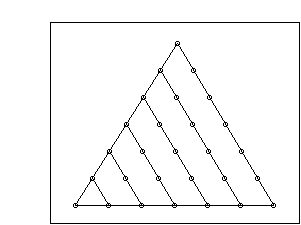
\includegraphics[scale=0.5]{triangular}
\caption{$T_7 = 28$}
\end{figure}
In order to accomplish this, we can begin from the left in each row, and add balls going right until the condition is satisfied in the row we're constructing. If $N$ is triangular, this process will result in a complete equilateral triangle. Each ball in a given row has one ball below and to the left (except the bottom row), and the ball furthest to the right has an additional ball below and to the right. So each row has exactly one more ball than the row above it. 

Suppose no $n \in \mathbb Z$ satisfies $N = \sum_{k=1}^n k$. Then some row will necessarily be incomplete once all $N$ balls have been placed, since otherwise $N = \sum_{k=1}^n k$ for some $n \in \mathbb Z$. This contradicts our hypothesis that $N$ is triangular. Therefore there must be some $n \in \mathbb Z$ for which $N = \sum_{k=1}^n k$. 

$(\Longleftarrow)$ Now suppose $N = \sum_{k=1}^n k$ for some $n \in \mathbb Z$. Then, 
\[
N = 1 + 2 + \cdots + n.
\]
Place $k$ balls in each row $k$, starting with $k=1$, and align each row below each previous row, where each successive row has one more ball. Stop at $k=n$. The resulting array of balls will be an equilateral triangle. If we add up the number of balls in each row, we get $1 + 2 + \cdots + n$, which by hypothesis is $N$. So $N$ is triangular. 
\end{proof}

\noindent (b) A number is triangular if and only if it is of the form $\frac{n(n+1)} 2$ for some $n \in \mathbb Z$. 
\begin{proof} $(\Longrightarrow)$ Suppose $N \in \mathbb Z$ is triangular. Then as we have shown, there exists some $n \in \mathbb Z$ so that 
\begin{equation} \label{6.6}
N = 1 + 2 + \cdots + n.
\end{equation}
By additive commutativity, this is equivalent to 
\begin{equation} \label{6.7}
N = n + (n-1) + \cdots + 2 + 1.
\end{equation}
Adding each term of \ref{6.6} and \ref{6.7} gives
\begin{align*}
2N &= (n+1) + (n-1 + 2) + \cdots + (2+n-1) + (1+n) \\
&= (n+1) + (n+1) + \cdots + (n+1) + (n+1) \\
&= n(n+1).
\end{align*}
Therefore $N = \frac{n(n+1)}2$. 

$(\Longleftarrow)$ Suppose $N = \frac{n(n+1)}2$ for some $n \in \mathbb Z$. Reversing the above algebraic steps gives
\[
2N = 2(1 + 2 + \cdots + n),
\]
so $N = 1 + 2 + \cdots + n$, and as we've shown, this implies that $N$ is triangular. \end{proof}

\noindent (c) The sum of any two consecutive triangular numbers is a perfect square. 
\begin{proof} Two consecutive triangular numbers must be of the form $\frac{n(n+1)}2$ and $\frac{(n+1)(n+2)}2$. Their sum is thus: 
\begin{align*}
\frac{n(n+1)}2 + \frac{(n+1)(n+2)}2 &= \frac{n^2 + n}2 + \frac{n^2 + 3n + 2}{2}\\
&= \frac{2n^2 + 4n + 2}2 \\
&= n^2 + 2n + 1 \\
&=(n+1)^2.
\end{align*} 
\end{proof}

\noindent (d) We will define a \emph{pentagonal number} as one that can represent the number of vertices in a pentagonal graph with equal vertices on each side, and successively smaller pentagonal subgraphs embedded in the original graph so that all subgraphs share one corner vertex. The first four pentagonal numbers are displayed below. 

\begin{figure}
\centering
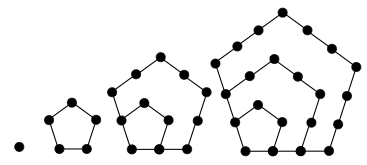
\includegraphics{pentagonal}
\caption{Pentagonal numbers}
\end{figure}

\end{problem}


\section{Homework 7}

\section{Homework 8}
\begin{problem}
A switchboard has ten cables that connect ten of the letters a through z to ten of the letters A through Z. How many ways are there to arrange the ten cables? For the purposes of this exercise,
note that $a\leftarrow B$ is different than $b\leftarrow A$.

\solution
The number of ways to choose 10 elements from $\{ a,. . ., z\}$ is 26 choose 10, i.e. ${26 \choose 10} = {\frac {26!}{16!10!}}= {5,311,735}$. Furthermore, the number of ways to choose 10 elements in $\{A,. . . , Z\}$, where order matters, is the number of permutations of 10 elements in a set of 26 elements: ${\frac {26!}{16!}}= {19,275,223,968,000}$. By multiplying these numbers we find that the number of ways to hook up the cables is $1.02384882*10^{20}$, or if you prefer, ${26 \choose 10}({\frac{26!}{16!}})$. 

\begin{problem}
I have three racks ($R_{1}$, $R_{2}$, and $R_{3}$), each of which holds 26 different hats. I’m planning on wearing
three hats today (it’s cold!), and I’m going to pick my first hat from $R_{1}$, my second hat from $R_{2}$,
and my third hat from $R_{3}$. How many ways can I wear my hats?

\solution
First, you have 26 different options. After making the first choice, there are 26 more options, so $26^{2}$. Finally, after making the second choice there are 26 more options for $R_{3}$. So $26^{3}$ is the number of options total.

\begin{problem}
It’s roughtly 50 years in the future. I’ve exhausted my hat combinations, and I want to mix things
up. If go truly crazy and pick my three daily hats from $R_{1}$, $R_{2}$, and $R_{3}$ in any order, how many
distinct hat combinations are possible? (Wearing hat A on top of hat B is different than wearing
hat B on top of hat A.)

\solution
There are $26^{3}$ different ways of choosing a hat from each rack (as shown by the previous problem). However, if the order of choosing the hats matters, there are more. Since each choice of 3 hats can be worn $3!=6$ different ways (which is the number of ways to permute the three hats), there are $6*26^{3}$ different options.


\section{Homework n+1}

\begin{problem}
Fill in the addition table below for the elliptic curve $E : y^2 = x^3 + 2x + 1$ over the finite field $\mathbb{F}_5$.

\solution
For points $(x_1, y_1)$ and $(x_2, y_2)$ on an elliptic curve $E= x^3 + ax + b$ over the finite field $\mathbb{F}_n$, If $x_1 = x_2$ and $y_1 \equiv -y_2$ (mod n), then $(x_1, y_1) + (x_2, y_2)$ = $\mathcal{O}$. Thus $(1,2) + (1,3) = (3,2) + (3,3) = (0,4) + (0,1) = \mathcal{O}$.

The equations to find $(x_1, y_1) + (x_2, y_2)  = (x_{3},y_{3})$ are as follows.
$$x_{3} = \lambda ^2 - x_{1} - x_{2}$$
$$y_{3}=\lambda(x_{1}-x_{3})-y_{1}$$

If $(x_1, y_1) = (x_2, y_2)$, then $ \lambda = (3x_{1}^2+A){(2y_{1})}^{-1}$.\\
Example: $(0,4) + (0,4)$.\\
$\lambda = (3(0)+2)(2(4))^{-1} = 2(8)^{-1} \equiv 2(3)^{-1} \equiv 2(2) = 4$ mod 5.\\
$x_{3} = 16-0-0 = 16 \equiv 1$ mod 5 and $y_{3}=4(0-1) - 4 = -8 \equiv 2$ mod 5.\\
Thus, $(0,4) + (0,4) = (1,2)$.\\

If $(x_1, y_1) \neq (x_2, y_2)$, then $ \lambda = (y_{2}-y_{1})(x_{2}-x_{1})^{-1}$.\\
Example: $(1,3) + (0,1)$.\\
$\lambda = (1-3)(0-1)^{-1}=(-2)(-1)^{-1} \equiv (3)(4)^{-1}= 3(4) = 12 \equiv 2$ mod 5.\\
$x_{3} = 4-1-0 = 3$ and $y_{3}= 2(1-3) -3 =2(-2)-3 = -7 \equiv 3$ mod 5.\\
Thus, $(1,3) + (0,1) = (3,3)$.\\

The addition table looks like...

\begin{tabular}{r|cccccc}
0 & (0,1) & (0,4) & (1,2) & (1,3) & (3,2) & (3,3)\\
\hline
(0,1) & (1,3) & $\mathcal{O}$ & (0,4) & (3,3) & (1,2) & (3,2)\\
(0,4) & $\mathcal{O}$ & (1,2) & (3,2) & (0,1) & (3,3) & (1,3) \\
(1,2) & (0,4) & (3,2) & (3,3) & $\mathcal{O}$ & (1,3) & (0,1)\\
(1,3) & (3,3) & (0,1) & $\mathcal{O}$ & (3,2) & (0,4) & (1,2)\\
(3,2) & (1,2) & (3,3) & (1,3) & (0,4) & (0,1) & $\mathcal{O}$ \\
(3,3) & (3,2) & (1,3) & (0,1) & (1,2) & $\mathcal{O}$ & (0,4)\\
\end{tabular}

\end{problem}
\begin{problem} 
This question refers to the elliptic curve $E : y^2 = x^3 + 2x + 1$ over the finite ring
$\mathbb{Z}/6\mathbb{Z} = \{0, 1, 2, 3, 4, 5\}$ mod 6.

\solution
a. List all 12 nonzero points on the curve E.

Note that in mod 6, $0^2\equiv0, 1^2\equiv1,2^2\equiv4, 3^2\equiv3, 4^2\equiv4,5^2\equiv1$.\\
Thus, if $y^2=1$, then $y=1$ or $y=5$.\\
Then we can make the following table.

\begin{tabular}{r|c|c}
x & $y^2$ & $(x,y)$ points\\
\hline
0 & 1 & (0,1), (0,5)\\
1 & 4 & (1,2), (1,4)\\
2 & 1 & (2,1), (2,5)\\
3 & 4 & (3,2), (3,4)\\
4 & 1 & (4,1), (4,5)\\
5 & 4 & (5,2), (5,4)\\
\end{tabular}

Thus the 12 nonzero points on the curve E are (0,1), (0,5), (1,2), (1,4), (2,1), (2,5), (3,2), (3,4), (4,1), (4,5), (5,2), and (5,4).

b. Let P = (2, 5). Use Lenstra’s algorithm (from Denise’s lecture on Monday) on the point P = (2, 5), and show that
this allows you to factor the number 6. 

$\lambda_{2P} = (3 \cdot 2^2 + 2)(2 \cdot 5)^{-1} = 14(10)^{-1} \equiv 2(4)^{-1} \equiv \frac{2}{4} = \frac{1}{2} = (2)^{-1}$.\\
Since 2 does not have an inverse mod 6, we have found a factor.\\
Thus, since $\frac{6}{2}=3$, $6=2\cdot3$.

\end{problem}
\begin{problem}
Use Lenstra’s algorithm to factor n = 589 with the curve $E : y^2 = x^3 + 4x + 9$ and the point $P = (2, 5)$.

\solution
a. Let x=2. Then $y^2 = 8+8+9=25 \equiv 1$. Since $y^2 = 5^2 \equiv 1$, point (2,5) exists.\\
b. Find P+P. Using the computer algorithm Professor Gibbon posted online, I calculated $P+P=(564,156)$.\\
c. Further, 
    $3P = (148,48)$\\
    $4P = (303,572)$\\
    $5P = (285,92)$\\
    $6P = (33,460)$\\
    Then, $7P$ produced an error message since the algorithm could not find an inverse.
    This is because the number was a factor of 589.\\
    Thus the error message produced that $589 = 31 \cdot 19$.
\end{problem}


\clearpage 

\glsaddall 
\printglossary

\begin{thebibliography}{9}
\bibitem{Singh} 
Simon Singh. 
\textit{The Code Book}. 
\end{thebibliography}
\end{document}
